% Options for packages loaded elsewhere
\PassOptionsToPackage{unicode}{hyperref}
\PassOptionsToPackage{hyphens}{url}
\PassOptionsToPackage{dvipsnames,svgnames*,x11names*}{xcolor}
%
\documentclass[
]{memoir}
\usepackage{amsmath,amssymb}
\usepackage{lmodern}
\usepackage{ifxetex,ifluatex}
\ifnum 0\ifxetex 1\fi\ifluatex 1\fi=0 % if pdftex
  \usepackage[T1]{fontenc}
  \usepackage[utf8]{inputenc}
  \usepackage{textcomp} % provide euro and other symbols
\else % if luatex or xetex
  \usepackage{unicode-math}
  \defaultfontfeatures{Scale=MatchLowercase}
  \defaultfontfeatures[\rmfamily]{Ligatures=TeX,Scale=1}
  \setmonofont[]{Inconsolata}
\fi
% Use upquote if available, for straight quotes in verbatim environments
\IfFileExists{upquote.sty}{\usepackage{upquote}}{}
\IfFileExists{microtype.sty}{% use microtype if available
  \usepackage[]{microtype}
  \UseMicrotypeSet[protrusion]{basicmath} % disable protrusion for tt fonts
}{}
\makeatletter
\@ifundefined{KOMAClassName}{% if non-KOMA class
  \IfFileExists{parskip.sty}{%
    \usepackage{parskip}
  }{% else
    \setlength{\parindent}{0pt}
    \setlength{\parskip}{6pt plus 2pt minus 1pt}}
}{% if KOMA class
  \KOMAoptions{parskip=half}}
\makeatother
\usepackage{xcolor}
\IfFileExists{xurl.sty}{\usepackage{xurl}}{} % add URL line breaks if available
\IfFileExists{bookmark.sty}{\usepackage{bookmark}}{\usepackage{hyperref}}
\hypersetup{
  pdftitle={Data Science per psicologi},
  pdfauthor={Corrado Caudek},
  colorlinks=true,
  linkcolor=Maroon,
  filecolor=Maroon,
  citecolor=Blue,
  urlcolor=Blue,
  pdfcreator={LaTeX via pandoc}}
\urlstyle{same} % disable monospaced font for URLs
\usepackage{color}
\usepackage{fancyvrb}
\newcommand{\VerbBar}{|}
\newcommand{\VERB}{\Verb[commandchars=\\\{\}]}
\DefineVerbatimEnvironment{Highlighting}{Verbatim}{commandchars=\\\{\}}
% Add ',fontsize=\small' for more characters per line
\usepackage{framed}
\definecolor{shadecolor}{RGB}{248,248,248}
\newenvironment{Shaded}{\begin{snugshade}}{\end{snugshade}}
\newcommand{\AlertTok}[1]{\textcolor[rgb]{0.94,0.16,0.16}{#1}}
\newcommand{\AnnotationTok}[1]{\textcolor[rgb]{0.56,0.35,0.01}{\textbf{\textit{#1}}}}
\newcommand{\AttributeTok}[1]{\textcolor[rgb]{0.77,0.63,0.00}{#1}}
\newcommand{\BaseNTok}[1]{\textcolor[rgb]{0.00,0.00,0.81}{#1}}
\newcommand{\BuiltInTok}[1]{#1}
\newcommand{\CharTok}[1]{\textcolor[rgb]{0.31,0.60,0.02}{#1}}
\newcommand{\CommentTok}[1]{\textcolor[rgb]{0.56,0.35,0.01}{\textit{#1}}}
\newcommand{\CommentVarTok}[1]{\textcolor[rgb]{0.56,0.35,0.01}{\textbf{\textit{#1}}}}
\newcommand{\ConstantTok}[1]{\textcolor[rgb]{0.00,0.00,0.00}{#1}}
\newcommand{\ControlFlowTok}[1]{\textcolor[rgb]{0.13,0.29,0.53}{\textbf{#1}}}
\newcommand{\DataTypeTok}[1]{\textcolor[rgb]{0.13,0.29,0.53}{#1}}
\newcommand{\DecValTok}[1]{\textcolor[rgb]{0.00,0.00,0.81}{#1}}
\newcommand{\DocumentationTok}[1]{\textcolor[rgb]{0.56,0.35,0.01}{\textbf{\textit{#1}}}}
\newcommand{\ErrorTok}[1]{\textcolor[rgb]{0.64,0.00,0.00}{\textbf{#1}}}
\newcommand{\ExtensionTok}[1]{#1}
\newcommand{\FloatTok}[1]{\textcolor[rgb]{0.00,0.00,0.81}{#1}}
\newcommand{\FunctionTok}[1]{\textcolor[rgb]{0.00,0.00,0.00}{#1}}
\newcommand{\ImportTok}[1]{#1}
\newcommand{\InformationTok}[1]{\textcolor[rgb]{0.56,0.35,0.01}{\textbf{\textit{#1}}}}
\newcommand{\KeywordTok}[1]{\textcolor[rgb]{0.13,0.29,0.53}{\textbf{#1}}}
\newcommand{\NormalTok}[1]{#1}
\newcommand{\OperatorTok}[1]{\textcolor[rgb]{0.81,0.36,0.00}{\textbf{#1}}}
\newcommand{\OtherTok}[1]{\textcolor[rgb]{0.56,0.35,0.01}{#1}}
\newcommand{\PreprocessorTok}[1]{\textcolor[rgb]{0.56,0.35,0.01}{\textit{#1}}}
\newcommand{\RegionMarkerTok}[1]{#1}
\newcommand{\SpecialCharTok}[1]{\textcolor[rgb]{0.00,0.00,0.00}{#1}}
\newcommand{\SpecialStringTok}[1]{\textcolor[rgb]{0.31,0.60,0.02}{#1}}
\newcommand{\StringTok}[1]{\textcolor[rgb]{0.31,0.60,0.02}{#1}}
\newcommand{\VariableTok}[1]{\textcolor[rgb]{0.00,0.00,0.00}{#1}}
\newcommand{\VerbatimStringTok}[1]{\textcolor[rgb]{0.31,0.60,0.02}{#1}}
\newcommand{\WarningTok}[1]{\textcolor[rgb]{0.56,0.35,0.01}{\textbf{\textit{#1}}}}
\usepackage{longtable,booktabs,array}
\usepackage{calc} % for calculating minipage widths
% Correct order of tables after \paragraph or \subparagraph
\usepackage{etoolbox}
\makeatletter
\patchcmd\longtable{\par}{\if@noskipsec\mbox{}\fi\par}{}{}
\makeatother
% Allow footnotes in longtable head/foot
\IfFileExists{footnotehyper.sty}{\usepackage{footnotehyper}}{\usepackage{footnote}}
\makesavenoteenv{longtable}
\usepackage{graphicx}
\makeatletter
\def\maxwidth{\ifdim\Gin@nat@width>\linewidth\linewidth\else\Gin@nat@width\fi}
\def\maxheight{\ifdim\Gin@nat@height>\textheight\textheight\else\Gin@nat@height\fi}
\makeatother
% Scale images if necessary, so that they will not overflow the page
% margins by default, and it is still possible to overwrite the defaults
% using explicit options in \includegraphics[width, height, ...]{}
\setkeys{Gin}{width=\maxwidth,height=\maxheight,keepaspectratio}
% Set default figure placement to htbp
\makeatletter
\def\fps@figure{htbp}
\makeatother
\setlength{\emergencystretch}{3em} % prevent overfull lines
\providecommand{\tightlist}{%
  \setlength{\itemsep}{0pt}\setlength{\parskip}{0pt}}
\setcounter{secnumdepth}{5}
\chapterstyle{bianchi}

\usepackage{mathtools}
\usepackage[italian]{babel} 
\usepackage{lmodern} 
\usepackage{booktabs}
\usepackage{hyperref}
\hypersetup{
  colorlinks=true
}
\usepackage[
  labelfont=bf, 
  font={small, it} 
]{caption} 
\usepackage{upquote} % print correct quotes in verbatim-environments
\usepackage[autostyle, italian=quotes]{csquotes}
\usepackage{empheq} 
\usepackage{xfrac}

\raggedbottom % allow variable (ragged) site heights
\frenchspacing
\setlength\parskip{1.5pt plus 1pt minus 0.5pt}


\DeclareMathOperator{\Var}{Var} % Define variance operator
\DeclareMathOperator{\SD}{SD} % Define sd operator
\DeclareMathOperator{\Cov}{Cov} % Define covariance operator
\DeclareMathOperator{\Corr}{Corr} % Define correlation operator
\DeclareMathOperator{\Me}{Me} % Define mediane operator
\DeclareMathOperator{\Mo}{Mo} % Define mode operator
\DeclareMathOperator{\Bin}{Bin} % Define binomial operator
\DeclareMathOperator{\Bernoulli}{Bernoulli} % Define Bernoulli operator
\DeclareMathOperator{\Poi}{Poi} % Define Poisson operator
\DeclareMathOperator{\Uniform}{Uniform} % Define Uniform operator
\DeclareMathOperator{\Cauchy}{Cauchy} % Define Cauchy operator
\DeclareMathOperator{\B}{\mathscr{B}} % Define Bernoulli operator
\newcommand{\R}{\textsf{R}} % Define R programming language symbol
\newcommand{\E}{\mathbb{E}} % Define expected value operator
\newcommand{\Real}{\mathbb{R}} % Define real number operator
\newcommand{\Prob}{\mathscr{P}}
\DeclareMathOperator*{\argmin}{arg\,min} % thin space, limits on side in displays
\DeclareMathOperator*{\argmax}{arg\,max} % thin space, limits on side in displays

\usepackage{microtype}

\usepackage{booktabs}
\usepackage{longtable}
\usepackage{array}
\usepackage{multirow}
\usepackage{wrapfig}
\usepackage{float}
\usepackage{colortbl}
\usepackage{pdflscape}
\usepackage{tabu}
\usepackage{threeparttable}
\usepackage{threeparttablex}
\usepackage[normalem]{ulem}
\usepackage{makecell}
\usepackage{xcolor}
\ifluatex
  \usepackage{selnolig}  % disable illegal ligatures
\fi
\usepackage[]{natbib}
\bibliographystyle{apalike}

\title{Data Science per psicologi}
\author{Corrado Caudek}
\date{2021-09-13}

\begin{document}
\maketitle

{
\hypersetup{linkcolor=}
\setcounter{tocdepth}{1}
\tableofcontents
}
\newpage

\vspace*{5cm}

\thispagestyle{empty}

\hypertarget{approssimazione-della-distribuzione-a-posteriori}{%
\chapter{Approssimazione della distribuzione a posteriori}\label{approssimazione-della-distribuzione-a-posteriori}}

In generale, in un problema bayesiano i dati \(y\) provengono da una densità \(p(y \mid \theta)\) e al parametro \(\theta\) viene assegnata una densità a priori \(p(\theta)\). Dopo avere osservato un campione \(Y = y\), la funzione di verosimiglianza è uguale a \(\mathcal{L}(\theta) = p(y \mid \theta)\) e la densità a posteriori diventa

\begin{equation}
p(\theta \mid y) = \frac{p(\theta) \mathcal{L}(\theta)}{\int p(\theta) \mathcal{L}(\theta) d \theta}.
\end{equation}

Si noti che, quando usiamo il teorema di Bayes per calcolare la distribuzione a posteriori del parametro di un modello statistico, al denominatore troviamo un integrale. Se vogliamo trovare la distribuzione a posteriori con metodi analitici è necessario usare distribuzioni a priori coniugate per la verosimiglianza.
Per quanto ``semplice'' in termini formali, questo approccio, però, limita di molto le possibili scelte del ricercatore. Nel senso che non è sempre sensato, dal punto di vista teorico, utilizzare distribuzioni a priori coniugate per la verosimiglianza per i parametri di interesse. Però, se usiamo delle distribuzioni a priori non coniutate per la verosimiglianza, ci troviamo in una condizione nella quale, per determinare la distribuzione a posteriori, è necessario calcolare un integrale che, nella maggior parte dei casi, non si può risolvere analiticamente. In altre parole: è possibile ottenere analiticamenre la distribuzione a posteriori solo per alcune specifiche combinazioni di distribuzioni a priori e verosimiglianza, il che limita considerevolmente la flessibilità della modellizzazione.

Inoltre, i sommari della distribuzione a posteriori sono espressi come rapporto di integrali. Ad esempio, la media a posteriori di \(\theta\) è data da
\begin{equation}
\mathbb{E}(\theta \mid y) = \frac{\int \theta p(\theta) \mathcal{L}(\theta) d \theta}{\int p(\theta) \mathcal{L}(\theta) d \theta}.
\end{equation}
Il calcolo del valore atteso a posteriori richiede dunque la valutazione di due integrali, ciascuno dei quali non esprimibile in forma chiusa. Per questa ragione, la strada principale che viene seguita nella modellistica bayesiana è quella che porta a determinare la distribuzione a posteriori non per via analitica, ma bensì mediante metodi numerici. La simulazione fornisce dunque la strategia generale del calcolo bayesiano.

A questo fine vengono usati i metodi di campionamento detti Monte-Carlo Markov-Chain (MCMC). Tali metodi costituiscono una potente e praticabile alternativa per la costruzione della distribuzione a posteriori per modelli complessi e consentono di decidere quali distribuzioni a priori e quali distribuzioni di verosimiglianza usare sulla base di considerazioni teoriche soltanto, senza dovere preoccuparsi di altri vincoli.

Dato che è basata su metodi computazionalmente intensivi, la stima numerica della funzione a posteriori può essere svolta soltanto mediante software. In anni recenti i metodi Bayesiani di analisi dei dati sono diventati sempre più popolari proprio perché la potenza di calcolo necessaria per svolgere tali calcoli è ora alla portata di tutti. Questo non era vero solo pochi decenni fa.

In questo Capitolo vedremo come sia possibile calcolare in maniera approssimata la distribuzione a posteriori. Presenteremo tre diverse tecniche che possono essere utilizzate a questo scopo:

\begin{enumerate}
\def\labelenumi{\arabic{enumi}.}
\tightlist
\item
  il metodo basato su griglia,
\item
  il metodo dell'approssimazione quadratica,
\item
  il metodo di Monte Carlo basato su Catena di Markov (MCMC).
\end{enumerate}

\hypertarget{metodo-basato-su-griglia}{%
\section{Metodo basato su griglia}\label{metodo-basato-su-griglia}}

Il metodo basato su griglia (\emph{grid-based}) è un metodo di approsimazione numerica basato su una griglia di punti uniformemente spaziati. Anche se la maggior parte dei parametri è continua (ovvero, in linea di principio ciascun parametro può assumere un numero infinito di valori), possiamo ottenere un'eccellente approssimazione della distribuzione a posteriori considerando solo una griglia finita di valori dei parametri. In un tale metodo, la densità di probabilità a posteriori può dunque essere approssimata tramite le densità di probabilità cacolate in ciascuna cella della griglia.

Il metodo basato su griglia si sviluppa in quattro fasi:

\begin{itemize}
\tightlist
\item
  Fissare una griglia discreta di possibili valori \(\theta\).\footnote{È chiaro che, per ottenere buone approssimazioni, è necessaria una griglia molto densa.}
\item
  Valutare la distribuzione a priori \(p(\theta)\) e la funzione di verosimiglianza \(\mathcal{L}(y \mid \theta)\) in corrispondenza di ciascun valore \(\theta\) della griglia.
\item
  Ottenere un'approssimazione discreta della densità a posteriori: (a) calcolare il prodotto \(p(\theta) \mathcal{L} (y \mid \theta)\) per ciascun
  valore \(\theta\) della griglia; e (b) normalizzare i prodotti così ottenuti in modo tale che la loro somma sia 1.
\item
  Selezionare \(N\) valori casuali della griglia in modo tale da ottenere un campione casuale delle densità a posteriori normalizzate.
\end{itemize}

\hypertarget{modello-beta-binomiale}{%
\subsection{Modello Beta-Binomiale}\label{modello-beta-binomiale}}

Supponiamo di avere osservato 9 sucessi in 10 prove Bernoulliane indipendenti.\footnote{La discussione del modello Beta-Binomiale segue molto da vicino la presentazione di \citet{Johnson2022bayesrules} utilizzando anche lo stesso codice \R.} Imponiamo alla distribuzione a priori su \(\theta\) (proabilità di successo in una singola prova) una Beta(2, 2) per descrivere la nostra incertezza sul parametro prima di avere osservato i dati. Dunque, il modello diventa:

\begin{align}
Y \mid \theta & \sim \text{Bin}(10, \pi) \notag\\
\theta & \sim \mbox{Beta}(2, 2).
\end{align}
In queste circostanze, l'aggiornamento bayesiano produce una distribuzione a posteriori Beta di parametri 11 (\(y + \alpha\) = 9 + 2) e 3 (\(n - y + \beta\) = 10 - 9 + 2):

\begin{equation}
\theta \mid (y = 9) \sim \mbox{Beta}(11, 3) \; .
\end{equation}

Per approssimare la distribuzione a posteriori, fissiamo una griglia di \(n = 6\) valori equispaziati: \(\theta \in \{0, 0.2, 0.4, 0.6, 0.8, 1\}\) (in seguito aumenteremo \(n\)):

\begin{Shaded}
\begin{Highlighting}[]
\NormalTok{grid\_data }\OtherTok{\textless{}{-}} \FunctionTok{tibble}\NormalTok{(}
  \AttributeTok{theta\_grid =} \FunctionTok{seq}\NormalTok{(}\AttributeTok{from =} \DecValTok{0}\NormalTok{, }\AttributeTok{to =} \DecValTok{1}\NormalTok{, }\AttributeTok{length =} \DecValTok{6}\NormalTok{)}
\NormalTok{)}
\end{Highlighting}
\end{Shaded}

\noindent
In corrispondenza di ciascun valore della griglia, valutiamo la distribuzione a priori \(\mbox{Beta}(2, 2)\) e la verosimiglianza \(\Bin(10, \theta)\) con \(y = 9\).

\begin{Shaded}
\begin{Highlighting}[]
\NormalTok{grid\_data }\OtherTok{\textless{}{-}}\NormalTok{ grid\_data }\SpecialCharTok{\%\textgreater{}\%}
  \FunctionTok{mutate}\NormalTok{(}
    \AttributeTok{prior =} \FunctionTok{dbeta}\NormalTok{(theta\_grid, }\DecValTok{2}\NormalTok{, }\DecValTok{2}\NormalTok{),}
    \AttributeTok{likelihood =} \FunctionTok{dbinom}\NormalTok{(}\DecValTok{9}\NormalTok{, }\DecValTok{10}\NormalTok{, theta\_grid)}
\NormalTok{  )}
\end{Highlighting}
\end{Shaded}

\noindent
In ciascuna cella della griglia, calcoliamo il prodotto della verosimiglianza e della distribuzione a priori. Troviamo così un'approssimazione discreta e non normalizzata della distribuzione a posteriori (\texttt{unnormalized}). Normalizziamo poi questa approssimazione dividendo ciascun valore del vettore \texttt{unnormalized} per la somma di tutti i valori del vettore:

\begin{Shaded}
\begin{Highlighting}[]
\NormalTok{grid\_data }\OtherTok{\textless{}{-}}\NormalTok{ grid\_data }\SpecialCharTok{\%\textgreater{}\%}
  \FunctionTok{mutate}\NormalTok{(}
    \AttributeTok{unnormalized =}\NormalTok{ likelihood }\SpecialCharTok{*}\NormalTok{ prior,}
    \AttributeTok{posterior =}\NormalTok{ unnormalized }\SpecialCharTok{/} \FunctionTok{sum}\NormalTok{(unnormalized))}
\end{Highlighting}
\end{Shaded}

\noindent
La somma dei valori così trovati è uguale a 1:

\begin{Shaded}
\begin{Highlighting}[]
\NormalTok{grid\_data }\SpecialCharTok{\%\textgreater{}\%}
  \FunctionTok{summarize}\NormalTok{(}
    \FunctionTok{sum}\NormalTok{(unnormalized),}
    \FunctionTok{sum}\NormalTok{(posterior)}
\NormalTok{  )}
\CommentTok{\#\textgreater{} \# A tibble: 1 x 2}
\CommentTok{\#\textgreater{}   \textasciigrave{}sum(unnormalized)\textasciigrave{} \textasciigrave{}sum(posterior)\textasciigrave{}}
\CommentTok{\#\textgreater{}                 \textless{}dbl\textgreater{}            \textless{}dbl\textgreater{}}
\CommentTok{\#\textgreater{} 1               0.318                1}
\end{Highlighting}
\end{Shaded}

\noindent
Abbiamo dunque ottenuto la seguente distribuzione a posteriori discretizzata \(p(\theta \mid y)\):

\begin{Shaded}
\begin{Highlighting}[]
\FunctionTok{round}\NormalTok{(grid\_data, }\DecValTok{2}\NormalTok{)}
\CommentTok{\#\textgreater{} \# A tibble: 6 x 5}
\CommentTok{\#\textgreater{}   theta\_grid prior likelihood unnormalized posterior}
\CommentTok{\#\textgreater{}        \textless{}dbl\textgreater{} \textless{}dbl\textgreater{}      \textless{}dbl\textgreater{}        \textless{}dbl\textgreater{}     \textless{}dbl\textgreater{}}
\CommentTok{\#\textgreater{} 1        0    0          0            0         0   }
\CommentTok{\#\textgreater{} 2        0.2  0.96       0            0         0   }
\CommentTok{\#\textgreater{} 3        0.4  1.44       0            0         0.01}
\CommentTok{\#\textgreater{} 4        0.6  1.44       0.04         0.06      0.18}
\CommentTok{\#\textgreater{} 5        0.8  0.96       0.27         0.26      0.81}
\CommentTok{\#\textgreater{} 6        1    0          0            0         0}
\end{Highlighting}
\end{Shaded}

\noindent
La figura \ref{fig:grid-method-6points-posterior-plot} mostra un grafico della distribuzione a posteriori discretizzata che è stata ottenuta:

\begin{Shaded}
\begin{Highlighting}[]
\NormalTok{grid\_data }\SpecialCharTok{\%\textgreater{}\%} 
  \FunctionTok{ggplot}\NormalTok{(}
    \FunctionTok{aes}\NormalTok{(}\AttributeTok{x =}\NormalTok{ theta\_grid, }\AttributeTok{y =}\NormalTok{ posterior)}
\NormalTok{  ) }\SpecialCharTok{+}
  \FunctionTok{geom\_point}\NormalTok{() }\SpecialCharTok{+}
  \FunctionTok{geom\_segment}\NormalTok{(}
    \FunctionTok{aes}\NormalTok{(}
      \AttributeTok{x =}\NormalTok{ theta\_grid, }
      \AttributeTok{xend =}\NormalTok{ theta\_grid, }
      \AttributeTok{y =} \DecValTok{0}\NormalTok{, }
      \AttributeTok{yend =}\NormalTok{ posterior)}
\NormalTok{  )}
\end{Highlighting}
\end{Shaded}

\begin{figure}

{\centering 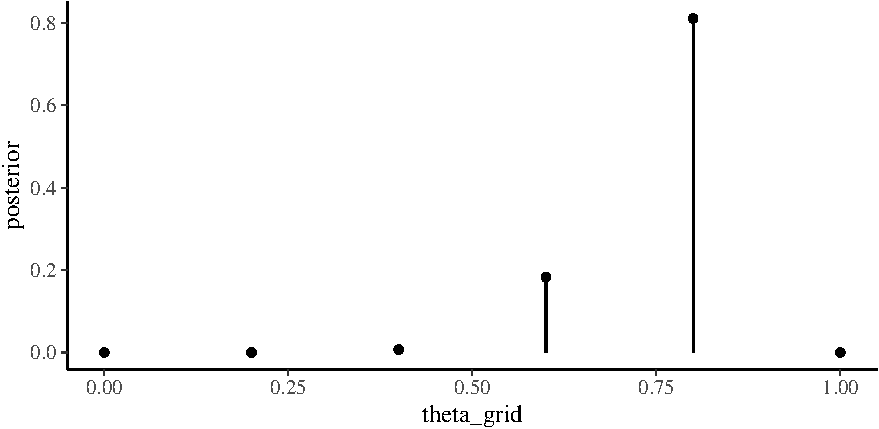
\includegraphics{035_approx_posterior_files/figure-latex/grid-method-6points-posterior-plot-1} 

}

\caption{Distribuzione a posteriori discretizzata ottenuta con il metodo grid-based per $y$ = 9 successi in 10 prove Bernoulliane, con distribuzione a priori $\mbox{Beta}(2, 2)$. È stata utilizzata una griglia di solo $n$ = 6 punti.}\label{fig:grid-method-6points-posterior-plot}
\end{figure}

\noindent
L'ultimo passo della simulazione è il campionamento dalla distribuzione a posteriori discretizzata:

\begin{Shaded}
\begin{Highlighting}[]
\FunctionTok{set.seed}\NormalTok{(}\DecValTok{84735}\NormalTok{)}
\NormalTok{post\_sample }\OtherTok{\textless{}{-}} \FunctionTok{sample\_n}\NormalTok{(}
\NormalTok{  grid\_data,}
  \AttributeTok{size =} \FloatTok{1e5}\NormalTok{,}
  \AttributeTok{weight =}\NormalTok{ posterior,}
  \AttributeTok{replace =} \ConstantTok{TRUE}
\NormalTok{)}
\end{Highlighting}
\end{Shaded}

\noindent
È facile intuire che i valori estratti con rimessa dalla distribuzione a posteriori discretizzata saranno quasi sempre uguali a 0.6 o 0.8. Questa intuizione è confermata dal grafico \ref{fig:grid-method-6points-posterior-plot-sampling} a cui è stata sovrapposta la vera distribuzione a posteriori \(\mbox{Beta}(11, 3)\):

\begin{Shaded}
\begin{Highlighting}[]
\FunctionTok{ggplot}\NormalTok{(post\_sample, }\FunctionTok{aes}\NormalTok{(}\AttributeTok{x =}\NormalTok{ theta\_grid)) }\SpecialCharTok{+}
  \FunctionTok{geom\_histogram}\NormalTok{(}\FunctionTok{aes}\NormalTok{(}\AttributeTok{y =}\NormalTok{ ..density..), }\AttributeTok{color =} \StringTok{"white"}\NormalTok{) }\SpecialCharTok{+}
  \FunctionTok{stat\_function}\NormalTok{(}\AttributeTok{fun =}\NormalTok{ dbeta, }\AttributeTok{args =} \FunctionTok{list}\NormalTok{(}\DecValTok{11}\NormalTok{, }\DecValTok{3}\NormalTok{)) }\SpecialCharTok{+}
  \FunctionTok{lims}\NormalTok{(}\AttributeTok{x =} \FunctionTok{c}\NormalTok{(}\DecValTok{0}\NormalTok{, }\DecValTok{1}\NormalTok{))}
\end{Highlighting}
\end{Shaded}

\begin{figure}

{\centering 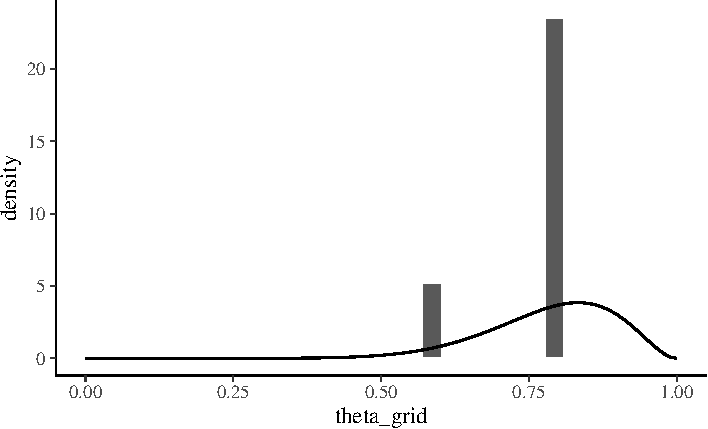
\includegraphics{035_approx_posterior_files/figure-latex/grid-method-6points-posterior-plot-sampling-1} 

}

\caption{Campionamento dalla  distribuzione a posteriori discretizzata ottenuta con il metodo grid-based per $y$ = 9 successi in 10 prove Bernoulliane, con distribuzione a priori $\mbox{Beta}(2, 2)$. È stata utilizzata una griglia di solo $n$ = 6 punti.}\label{fig:grid-method-6points-posterior-plot-sampling}
\end{figure}

\noindent
La figura \ref{fig:grid-method-6points-posterior-plot-sampling} mostra che, con una griglia così sparsa abbiamo ottenuto una versione estremamente approssimata della vera distribuzione a posteriori. Possiamo ottenere un risultato migliore con una griglia più densa, come indicato nella figura \ref{fig:grid-method-100points-posterior-plot-sampling}:

\begin{Shaded}
\begin{Highlighting}[]
\NormalTok{grid\_data  }\OtherTok{\textless{}{-}} \FunctionTok{tibble}\NormalTok{(}
  \AttributeTok{theta\_grid =} \FunctionTok{seq}\NormalTok{(}\AttributeTok{from =} \DecValTok{0}\NormalTok{, }\AttributeTok{to =} \DecValTok{1}\NormalTok{, }\AttributeTok{length.out =} \DecValTok{100}\NormalTok{)}
\NormalTok{)}

\NormalTok{grid\_data }\OtherTok{\textless{}{-}}\NormalTok{ grid\_data }\SpecialCharTok{\%\textgreater{}\%}
  \FunctionTok{mutate}\NormalTok{(}
    \AttributeTok{prior =} \FunctionTok{dbeta}\NormalTok{(theta\_grid, }\DecValTok{2}\NormalTok{, }\DecValTok{2}\NormalTok{),}
    \AttributeTok{likelihood =} \FunctionTok{dbinom}\NormalTok{(}\DecValTok{9}\NormalTok{, }\DecValTok{10}\NormalTok{, theta\_grid)}
\NormalTok{  )}

\NormalTok{grid\_data }\OtherTok{\textless{}{-}}\NormalTok{ grid\_data }\SpecialCharTok{\%\textgreater{}\%}
  \FunctionTok{mutate}\NormalTok{(}
    \AttributeTok{unnormalized =}\NormalTok{ likelihood }\SpecialCharTok{*}\NormalTok{ prior,}
    \AttributeTok{posterior =}\NormalTok{ unnormalized }\SpecialCharTok{/} \FunctionTok{sum}\NormalTok{(unnormalized)}
\NormalTok{  )}

\NormalTok{grid\_data }\SpecialCharTok{\%\textgreater{}\%} 
\FunctionTok{ggplot}\NormalTok{(}
  \FunctionTok{aes}\NormalTok{(}\AttributeTok{x =}\NormalTok{ theta\_grid, }\AttributeTok{y =}\NormalTok{ posterior)}
\NormalTok{) }\SpecialCharTok{+}
  \FunctionTok{geom\_point}\NormalTok{() }\SpecialCharTok{+}
  \FunctionTok{geom\_segment}\NormalTok{(}
    \FunctionTok{aes}\NormalTok{(}
      \AttributeTok{x =}\NormalTok{ theta\_grid, }
      \AttributeTok{xend =}\NormalTok{ theta\_grid, }
      \AttributeTok{y =} \DecValTok{0}\NormalTok{, }
      \AttributeTok{yend =}\NormalTok{ posterior)}
\NormalTok{  )}
\end{Highlighting}
\end{Shaded}

\begin{figure}

{\centering 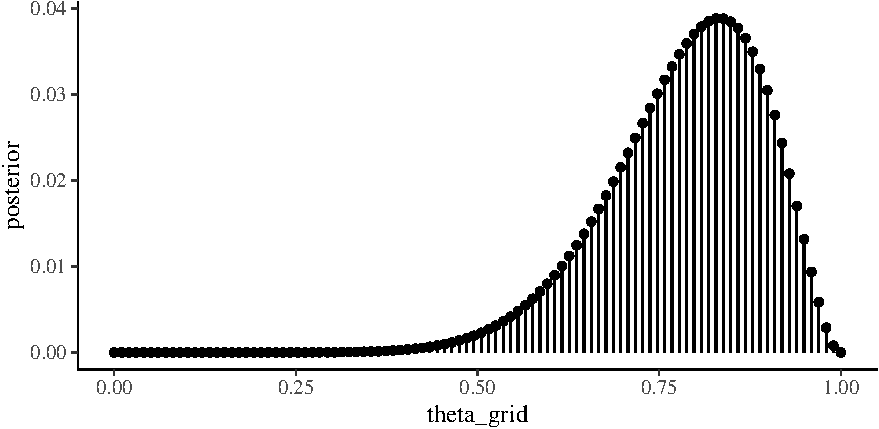
\includegraphics{035_approx_posterior_files/figure-latex/grid-method-100points-posterior-plot-sampling-1} 

}

\caption{Distribuzione a posteriori discretizzata ottenuta con il metodo grid-based per $y$ = 9 successi in 10 prove Bernoulliane, con distribuzione a priori $\mbox{Beta}(2, 2)$. È stata utilizzata una griglia di $n$ = 100 punti.}\label{fig:grid-method-100points-posterior-plot-sampling}
\end{figure}

\noindent
Campioniamo ora 10000 punti:

\begin{Shaded}
\begin{Highlighting}[]
\CommentTok{\# Set the seed}
\FunctionTok{set.seed}\NormalTok{(}\DecValTok{84735}\NormalTok{)}
\NormalTok{post\_sample }\OtherTok{\textless{}{-}} \FunctionTok{sample\_n}\NormalTok{(}
\NormalTok{  grid\_data,}
  \AttributeTok{size =} \FloatTok{1e4}\NormalTok{,}
  \AttributeTok{weight =}\NormalTok{ posterior,}
  \AttributeTok{replace =} \ConstantTok{TRUE}
\NormalTok{)}
\end{Highlighting}
\end{Shaded}

\noindent
Con il campionamento dalla distribuzione a posteriori discretizzata costruita mediante una griglia più densa (\(n = 100\)) otteniamo un risultato soddisfacente (figura \ref{fig:grid-method-100points-posterior-plot-and-correct-posterior}): la distribuzione dei valori prodotti dalla simulazione ora approssima molto bene la corretta distribuzione a posteriori \(p(\theta \mid y) = \mbox{Beta}(11, 3)\).

\begin{Shaded}
\begin{Highlighting}[]
\NormalTok{post\_sample }\SpecialCharTok{\%\textgreater{}\%}
  \FunctionTok{ggplot}\NormalTok{(}\FunctionTok{aes}\NormalTok{(}\AttributeTok{x =}\NormalTok{ theta\_grid)) }\SpecialCharTok{+}
  \FunctionTok{geom\_histogram}\NormalTok{(}
    \FunctionTok{aes}\NormalTok{(}\AttributeTok{y =}\NormalTok{ ..density..), }
    \AttributeTok{color =} \StringTok{"white"}\NormalTok{, }
    \AttributeTok{binwidth =} \FloatTok{0.05}
\NormalTok{  ) }\SpecialCharTok{+}
  \FunctionTok{stat\_function}\NormalTok{(}\AttributeTok{fun =}\NormalTok{ dbeta, }\AttributeTok{args =} \FunctionTok{list}\NormalTok{(}\DecValTok{11}\NormalTok{, }\DecValTok{3}\NormalTok{)) }\SpecialCharTok{+}
  \FunctionTok{lims}\NormalTok{(}\AttributeTok{x =} \FunctionTok{c}\NormalTok{(}\DecValTok{0}\NormalTok{, }\DecValTok{1}\NormalTok{))}
\end{Highlighting}
\end{Shaded}

\begin{figure}

{\centering 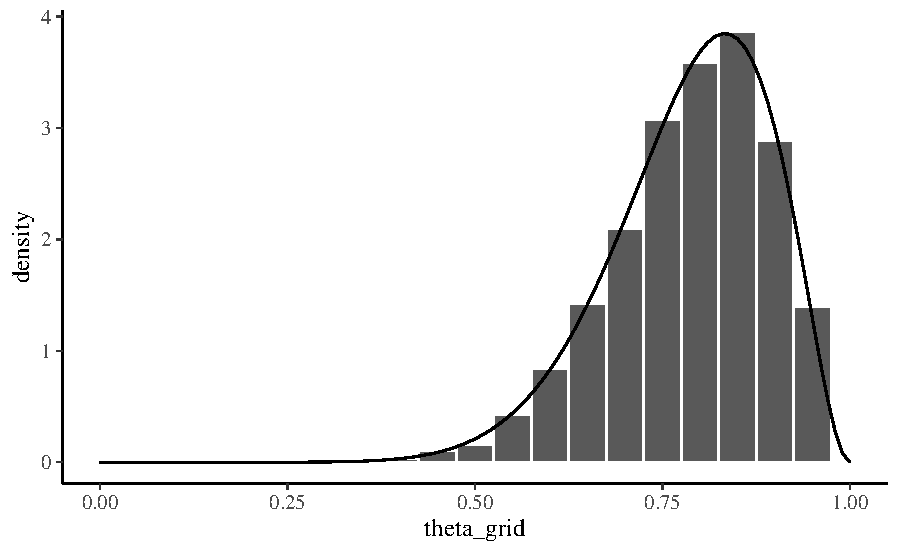
\includegraphics{035_approx_posterior_files/figure-latex/grid-method-100points-posterior-plot-and-correct-posterior-1} 

}

\caption{Campionamento dalla  distribuzione a posteriori discretizzata ottenuta con il metodo grid-based per $y$ = 9 successi in 10 prove Bernoulliane, con distribuzione a priori $\mbox{Beta}(2, 2)$. È stata utilizzata una griglia di $n$ = 100 punti. All'istogramma è stata sovrapposta lacorretta distribuzione a posteriori, ovvero la densità $\mbox{Beta}(11, 3)$.}\label{fig:grid-method-100points-posterior-plot-and-correct-posterior}
\end{figure}

Possiamo concludere dicendo che il metodo basato su griglia è molto intuitivo e non richiede particolari competenze di programmazione per essere implementato. Inoltre, fornisce un risultato che, per tutti gli scopi pratici, può essere considerato come un campione casuale estratto da \(p(\theta \mid y)\). Tuttavia, anche se tale metodo fornisce risultati accuratissimi, esso ha un uso limitato. A causa della \emph{maledizione della dimensionalità}\footnote{Che cos'è la \emph{maledizione della dimensionalità}? È molto facile da capire. Supponiamo di utilizzare una griglia di 100 punti equispaziati. Nel caso di un solo parametro, sarà necessario calcolare 100 valori. Per due parametri devono essere calcolari \(100^2\) valori. Ma già per 10 parametri avremo bisogno di calcolare \(10^{10}\) valori -- è facile capire che una tale quantità di calcoli è troppo grande anche per un computer molto potente. Per modelli che richiedono la stima di un numero non piccolo di parametri è dunque necessario procedere in un altro modo.}, infatti, il metodo basato su griglia può essere solo usato nel caso di semplici modelli statistici, con non più di due parametri. Nella pratica concreta tale metodo viene dunque sostituito da altre tecniche più efficienti in quanto, anche nei più comuni modelli utilizzati in psicologia, vengono solitamente stimati centinaia se non migliaia di parametri.

\hypertarget{approssimazione-quadratica}{%
\section{Approssimazione quadratica}\label{approssimazione-quadratica}}

L'approssimazione quadratica è uno dei metodi che possono essere usati per superare il problema della ``maledizione della dimensionalità''. La motivazione di tale metodo è la seguente. Sappiamo che, in generale, la regione della distribuzione a posteriori che si trova in prossimità del suo massimo può essere ben approssimata dalla forma di una distribuzione Normale.\footnote{Descrivere la distribuzione a posteriori mediante la distribuzione Normale significa utilizzare un'approssimazione che viene, appunto, chiamata ``quadratica'' (tale approssimazione si dice quadratica perché il logaritmo di una distribuzione gaussiana forma una parabola e la parabola è una funzione quadratica -- dunque, mediante questa approssimazione descriviamo il logaritmo della distribuzione a posteriori mediante una parabola).}

L'approssimazione quadratica si pone due obiettivi.

\begin{enumerate}
\def\labelenumi{\arabic{enumi}.}
\item
  Trovare la moda della distribuzione a posteriori. Ci sono varie
  procedure di ottimizzazione, implementate in \(\R\), in
  grado di trovare il massimo di una distribuzione.
\item
  Stimare la curvatura della distribuzione in prossimità della moda.
  Una stima della curvatura è sufficiente per trovare
  un'approssimazione quadratica dell'intera distribuzione. In alcuni
  casi, questi calcoli possono essere fatti seguendo una procedura
  analitica, ma solitamente vengono usate delle tecniche numeriche.
\end{enumerate}

Una descrizione della distribuzione a posteriori ottenuta mediante l'approssimazione quadratica si ottiene mediante la funzione \texttt{quap()} contenuta nel pacchetto \texttt{rethinking}:\footnote{Il pacchetto \texttt{rethinking} è stato creato da \citet{McElreath_rethinking} per accompagnare il suo testo \emph{Statistical Rethinking}\(^2\). Per l'installazione si veda \url{https://github.com/rmcelreath/rethinking}.}

\begin{Shaded}
\begin{Highlighting}[]
\FunctionTok{suppressPackageStartupMessages}\NormalTok{(}\FunctionTok{library}\NormalTok{(}\StringTok{"rethinking"}\NormalTok{))}

\NormalTok{mod }\OtherTok{\textless{}{-}} \FunctionTok{quap}\NormalTok{(}
  \FunctionTok{alist}\NormalTok{(}
\NormalTok{  N }\SpecialCharTok{\textasciitilde{}} \FunctionTok{dbinom}\NormalTok{(N }\SpecialCharTok{+}\NormalTok{ P, p), }\CommentTok{\# verosimiglianza binomiale}
\NormalTok{  p }\SpecialCharTok{\textasciitilde{}} \FunctionTok{dbeta}\NormalTok{(}\DecValTok{2}\NormalTok{, }\DecValTok{10}\NormalTok{) }\CommentTok{\# distribuzione a priori Beta(2, 10)}
\NormalTok{  ),}
  \AttributeTok{data =} \FunctionTok{list}\NormalTok{(}\AttributeTok{N =} \DecValTok{23}\NormalTok{, }\AttributeTok{P =} \DecValTok{7}\NormalTok{)}
\NormalTok{)}
\end{Highlighting}
\end{Shaded}

Un sommario dell'approssimazione quadratica è fornito da

\begin{Shaded}
\begin{Highlighting}[]
\FunctionTok{precis}\NormalTok{(mod, }\AttributeTok{prob =} \FloatTok{0.95}\NormalTok{)}
\CommentTok{\#\textgreater{}        mean        sd      2.5\%     97.5\%}
\CommentTok{\#\textgreater{} p 0.5999999 0.0774593 0.4481824 0.7518173}
\end{Highlighting}
\end{Shaded}

Qui sotto è fornito un confronto tra la corretta distribuzione a posteriori (linea continua) e l'approssimazione quadratica (linea trateggiata).

\begin{Shaded}
\begin{Highlighting}[]
\NormalTok{N }\OtherTok{\textless{}{-}} \DecValTok{23}
\NormalTok{P }\OtherTok{\textless{}{-}} \DecValTok{7}
\NormalTok{a }\OtherTok{\textless{}{-}}\NormalTok{ N }\SpecialCharTok{+} \DecValTok{2}
\NormalTok{b }\OtherTok{\textless{}{-}}\NormalTok{ P }\SpecialCharTok{+} \DecValTok{10}
\FunctionTok{curve}\NormalTok{(}\FunctionTok{dbeta}\NormalTok{(x, a, b), }\AttributeTok{from=}\DecValTok{0}\NormalTok{, }\AttributeTok{to=}\DecValTok{1}\NormalTok{, }\AttributeTok{ylab=}\StringTok{"Densità"}\NormalTok{)}
\CommentTok{\# approssimazione quadratica}
\FunctionTok{curve}\NormalTok{(}
  \FunctionTok{dnorm}\NormalTok{(x, a}\SpecialCharTok{/}\NormalTok{(a}\SpecialCharTok{+}\NormalTok{b), }\FunctionTok{sqrt}\NormalTok{((a}\SpecialCharTok{*}\NormalTok{b)}\SpecialCharTok{/}\NormalTok{((a}\SpecialCharTok{+}\NormalTok{b)}\SpecialCharTok{\^{}}\DecValTok{2}\SpecialCharTok{*}\NormalTok{(a}\SpecialCharTok{+}\NormalTok{b}\SpecialCharTok{+}\DecValTok{1}\NormalTok{)))),}
  \AttributeTok{lty =} \DecValTok{2}\NormalTok{,}
  \AttributeTok{add =} \ConstantTok{TRUE}
\NormalTok{)}
\end{Highlighting}
\end{Shaded}

\begin{center}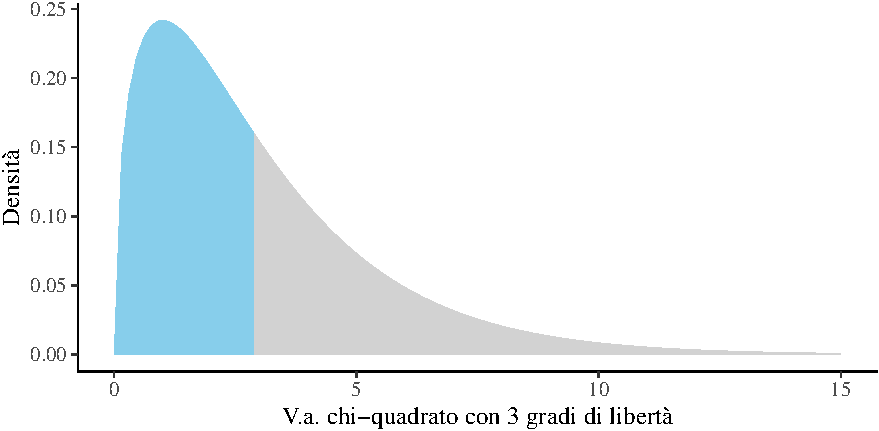
\includegraphics{035_approx_posterior_files/figure-latex/unnamed-chunk-10-1} \end{center}

Il grafico precedente mostra che l'approssimazione quadratica fornisce risultati soddisfacenti. Tali risultati sono simili (o identici) a quelli ottenuti con il metodo \emph{grid-based}, con il vantaggio aggiuntivo di disporre di una serie di funzioni \(\R\) in grado di svolgere i calcoli per noi. In realtà, però, l'approssimazione quadratica è poco usata perché, per problemi complessi, è più conveniente fare ricorso ai metodi Monte Carlo basati su Catena di Markov (MCMC) che verranno descritti nel Paragrafo successivo.

\hypertarget{chapter-simulazioneMC}{%
\section{Metodo Monte Carlo}\label{chapter-simulazioneMC}}

Una verosimiglianza Binomiale e una distribuzione a priori Beta producono una distribuzione a posteriori Beta (si veda il capitolo \ref{chapter-distr-priori-coniugate}). Con una simulazione \(\R\) è dunque facile ricavare dei campioni causali dalla distribuzione a posteriori. Maggiore è il numero di campioni, migliore sarà l'approssimazione della distribuzione a posteriori.

Continuando con l'esempio precedente,

\begin{align}
y \mid \theta, n &\sim \Bin(y = 23, n = 30 \mid \theta) \notag\\
\theta_{prior} &\sim \mbox{Beta}(2, 10) \notag\\
\theta_{post}  &\sim \mbox{Beta}(y + a = 23 + 2 = 25, n - y + b = 30 - 23 + 10 = 17), \notag
\end{align}

\noindent
stimiamo, ad esempio, il valore della media a posteriori di \(\theta\):

\begin{Shaded}
\begin{Highlighting}[]
\FunctionTok{set.seed}\NormalTok{(}\DecValTok{7543897}\NormalTok{)}
\FunctionTok{print}\NormalTok{(}\FunctionTok{mean}\NormalTok{(}\FunctionTok{rbeta}\NormalTok{(}\FloatTok{1e2}\NormalTok{, }\AttributeTok{shape1 =} \DecValTok{25}\NormalTok{, }\AttributeTok{shape2 =} \DecValTok{17}\NormalTok{)), }\DecValTok{6}\NormalTok{)}
\CommentTok{\#\textgreater{} [1] 0.587548}
\end{Highlighting}
\end{Shaded}

\noindent
L'approssimazione migliora all'aumentare del numero di campioni estratto dalla distribuzione a posteriori:

\begin{Shaded}
\begin{Highlighting}[]
\FunctionTok{print}\NormalTok{(}\FunctionTok{mean}\NormalTok{(}\FunctionTok{rbeta}\NormalTok{(}\FloatTok{1e3}\NormalTok{, }\AttributeTok{shape1 =} \DecValTok{25}\NormalTok{, }\AttributeTok{shape2 =} \DecValTok{17}\NormalTok{)), }\DecValTok{6}\NormalTok{)}
\CommentTok{\#\textgreater{} [1] 0.597659}
\end{Highlighting}
\end{Shaded}

\begin{Shaded}
\begin{Highlighting}[]
\FunctionTok{print}\NormalTok{(}\FunctionTok{mean}\NormalTok{(}\FunctionTok{rbeta}\NormalTok{(}\FloatTok{1e4}\NormalTok{, }\AttributeTok{shape1 =} \DecValTok{25}\NormalTok{, }\AttributeTok{shape2 =} \DecValTok{17}\NormalTok{)), }\DecValTok{6}\NormalTok{)}
\CommentTok{\#\textgreater{} [1] 0.595723}
\end{Highlighting}
\end{Shaded}

\begin{Shaded}
\begin{Highlighting}[]
\FunctionTok{print}\NormalTok{(}\FunctionTok{mean}\NormalTok{(}\FunctionTok{rbeta}\NormalTok{(}\FloatTok{1e5}\NormalTok{, }\AttributeTok{shape1 =} \DecValTok{25}\NormalTok{, }\AttributeTok{shape2 =} \DecValTok{17}\NormalTok{)), }\DecValTok{6}\NormalTok{)}
\CommentTok{\#\textgreater{} [1] 0.595271}
\end{Highlighting}
\end{Shaded}

\noindent
È lo stesso ragionamento che abbiamo fatto in riferiento alla relazione tra campione e popolazione: al crescere della numerosità campionaria il campione approssima sempre meglio le proprietà della popolazione da cui è stato estratto (legge dei grandi numeri). Nel caso presente, il risultato esatto è

\[
\bar{\theta}_{post} = \frac{\alpha}{\alpha + \beta} = \frac{25}{25 + 17} \approx 0.5952.
\]
\noindent
Quando il numero di campioni tratti dalla distribuzione a posteriori è molto grande, quindi, la distribuzione dei campioni converge alla densità della popolazione (si veda l'Appendice \ref{integration-mc}).\footnote{Si noti, naturalmente, che il numero dei campioni di simulazione è controllato dal ricercatore; è totalmente diverso dalla dimensione del campione che è fissa ed è una proprietà dei dati.}

Inoltre, le statistiche descrittive (es. media, moda, varianza, eccetera) dei campioni estratti dalla distribuzione a posteriori convergeranno ai corrispondenti valori della distribuzione a posteriori. La figura @ref\{fig:mcmc-chains-1\} mostra come, all'aumentare del numero di repliche, la media, la mediana, la deviazione standard e l'asimmetria convergono ai veri valori della distribuzione a posteriori (linee rosse tratteggiate).

\begin{figure}

{\centering 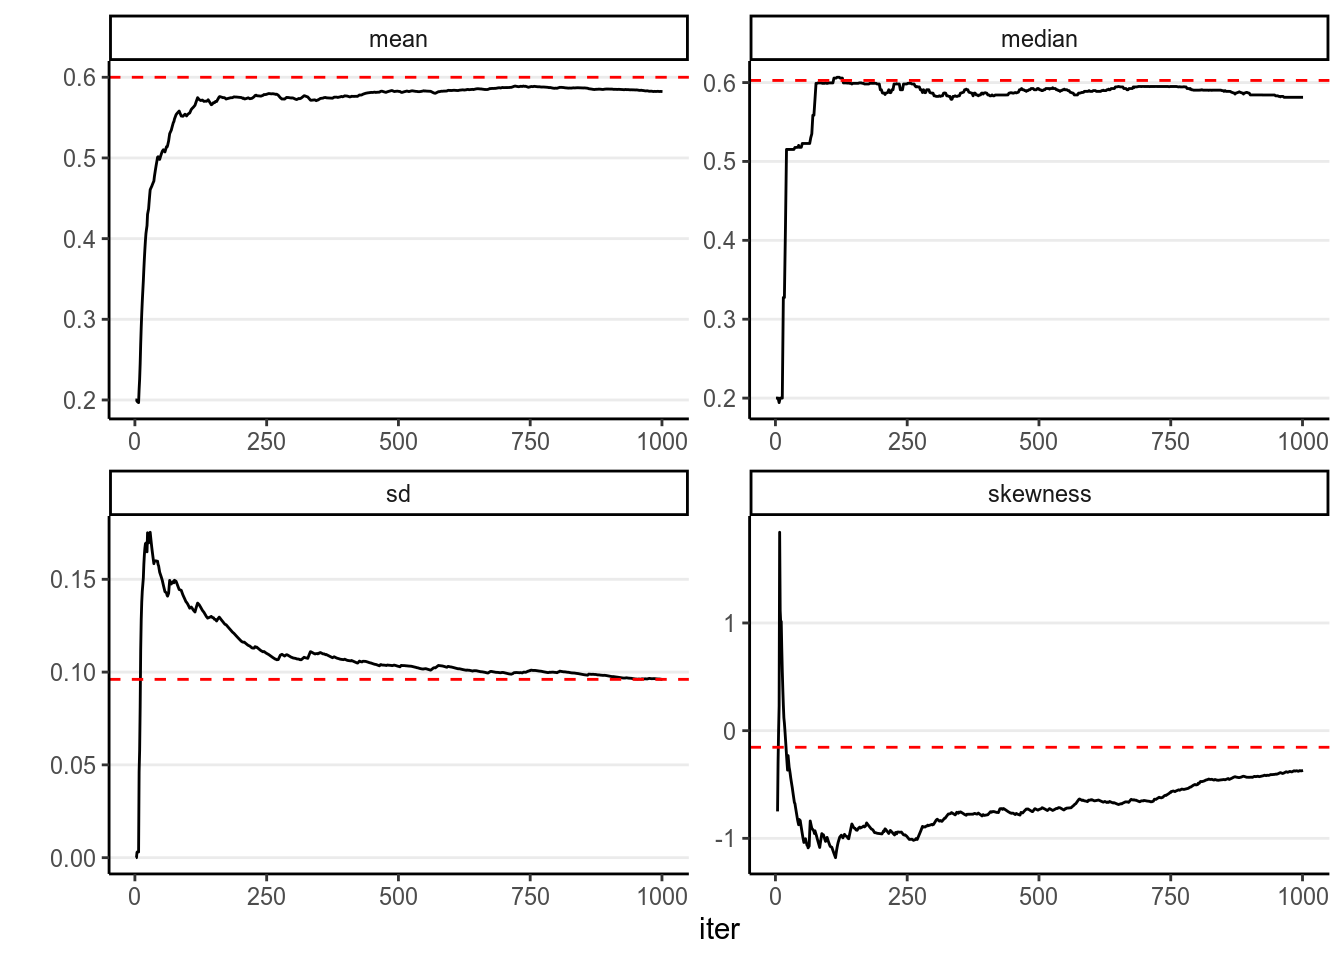
\includegraphics[width=0.8\linewidth]{/Users/corrado/Documents/teaching/2021-22/psicometria/dspp/images/mcmc-chains-1} 

}

\caption{Convergenza delle simulazioni Monte Carlo.}\label{fig:mcmc-chains-1}
\end{figure}

\hypertarget{metodi-mc-basati-su-catena-di-markov}{%
\section{Metodi MC basati su Catena di Markov}\label{metodi-mc-basati-su-catena-di-markov}}

Nel Paragrafo \ref{chapter-simulazioneMC} la simulazione Monte Carlo funzionava perché

\begin{enumerate}
\def\labelenumi{(\alph{enumi})}
\tightlist
\item
  sapevamo che la distribuzione a posteriori era una \(\mbox{Beta}(25, 17)\),
\item
  era possibile usare le funzioni \(\R\) per estrarre campioni casuali da tale distribuzione.
\end{enumerate}

\noindent
Tuttavia, capita raramente di usare una distribuzione a priori coniugata alla verosimiglianza, quindi in generale non valgono né la condizione (a) né la condizione (b) descritte sopra. Ad esempio, nel caso di una verosimiglianza binomiale e una distribuzione a priori Normale, la distribuzione a posteriori di \(\theta\) è

\[
p(\theta \mid y) = \frac{\mathrm{e}^{-(\theta - 1 / 2)^2} \theta^y (1 - \theta)^{n - y}} {\int_0^1 \mathrm{e}^{-(t - 1 / 2)^2} t^y (1 - t)^{n - y} dt}.
\]
\noindent
Una tale distribuzione non è implementata in \(\R\) e dunque non possiamo campionare da \(p(\theta \mid y)\).

Per fortuna, esiste un algoritmo chiamato Monte Carlo basato su catena di Markov (\emph{Markov Chain Monte Carlo}, MCMC) che consente il campionamento da una distribuzione a posteriori senza che sia necessario conoscere la rappresentazione analitica di una tale distribuzione. I metodi Monte Carlo basati su catena di Markov consentono di costruire sequenze di punti (le ``catene'') nello spazio dei parametri le cui densità sono proporzionali alla distribuzione a posteriori --- in altre parole, dopo aver simulato un grande numero di passi della catena si possono usare i valori così generati come se fossero un campione casuale della distribuzione a posteriori. Le tecniche MCMC sono attualmente il metodo computazionale maggiormente utilizzato per risolvere i problemi di inferenza bayesiana.

\hypertarget{catene-di-markov}{%
\subsection{Catene di Markov}\label{catene-di-markov}}

Per introdurre il concetto di catena di Markov, supponiamo che una persona esegua una passeggiata casuale sulla retta dei numeri naturali considerando solo i valori 1, 2, 3, 4, 5, 6.\footnote{Seguiamo qui la presentazione fornita da \href{https://github.com/bob-carpenter/prob-stats}{Bob Carpenter}.} Se la persona è collocata su un valore interno dei valori possibili (ovvero, 2, 3, 4 o 5), nel passo successivo è altrettanto probabile che rimanga su quel numero o si sposti su un numero adiacente. Se si muove, è ugualmente probabile che si muova a sinistra o a destra. Se la persona si trova su uno dei valori estremi (ovvero, 1 o 6), nel passo successivo è altrettanto probabile che rimanga rimanga su quel numero o si sposti nella posizione adiacente.

Questo è un esempio di una catena di Markov discreta. Una catena di Markov descrive il movimento probabilistico tra un numero di stati. Nell'esempio ci sono sei possibili stati, da 1 a 6, i quali corrispondono alle possibili posizioni della passeggiata casuale. Data la sua posizione corrente, la persona si sposterà nelle altre posizioni possibili con delle specifiche probabilità. La probabilità che si sposti in un'altra posizione dipende solo dalla sua posizione attuale e non dalle posizioni visitate in precedenza.

È possibile descrivere il movimento tra gli stati nei termini delle cosiddette \emph{probabilità di transizione}, ovvero le probabilità di movimento tra tutti i possibili stati in un unico passaggio di una catena di Markov. Le probabilità di transizione sono riassunte in una \emph{matrice di transizione} \(P\):

\begin{Shaded}
\begin{Highlighting}[]
\NormalTok{p }\OtherTok{\textless{}{-}} \FunctionTok{c}\NormalTok{(}\DecValTok{0}\NormalTok{, }\DecValTok{0}\NormalTok{, }\DecValTok{1}\NormalTok{, }\DecValTok{0}\NormalTok{, }\DecValTok{0}\NormalTok{, }\DecValTok{0}\NormalTok{)}

\NormalTok{P }\OtherTok{\textless{}{-}} \FunctionTok{matrix}\NormalTok{(}
  \FunctionTok{c}\NormalTok{(.}\DecValTok{5}\NormalTok{, .}\DecValTok{5}\NormalTok{, }\DecValTok{0}\NormalTok{, }\DecValTok{0}\NormalTok{, }\DecValTok{0}\NormalTok{, }\DecValTok{0}\NormalTok{,}
\NormalTok{    .}\DecValTok{25}\NormalTok{, .}\DecValTok{5}\NormalTok{, .}\DecValTok{25}\NormalTok{, }\DecValTok{0}\NormalTok{, }\DecValTok{0}\NormalTok{, }\DecValTok{0}\NormalTok{,}
    \DecValTok{0}\NormalTok{, .}\DecValTok{25}\NormalTok{, .}\DecValTok{5}\NormalTok{, .}\DecValTok{25}\NormalTok{, }\DecValTok{0}\NormalTok{, }\DecValTok{0}\NormalTok{,}
    \DecValTok{0}\NormalTok{, }\DecValTok{0}\NormalTok{, .}\DecValTok{25}\NormalTok{, .}\DecValTok{5}\NormalTok{, .}\DecValTok{25}\NormalTok{, }\DecValTok{0}\NormalTok{,}
    \DecValTok{0}\NormalTok{, }\DecValTok{0}\NormalTok{, }\DecValTok{0}\NormalTok{, .}\DecValTok{25}\NormalTok{, .}\DecValTok{5}\NormalTok{, .}\DecValTok{25}\NormalTok{,}
    \DecValTok{0}\NormalTok{, }\DecValTok{0}\NormalTok{, }\DecValTok{0}\NormalTok{, }\DecValTok{0}\NormalTok{, .}\DecValTok{5}\NormalTok{, .}\DecValTok{5}
\NormalTok{    ),}
  \AttributeTok{nrow =} \DecValTok{6}\NormalTok{, }\AttributeTok{ncol =} \DecValTok{6}\NormalTok{, }\AttributeTok{byrow =} \ConstantTok{TRUE}\NormalTok{)}

\NormalTok{kableExtra}\SpecialCharTok{::}\FunctionTok{kable}\NormalTok{(P)}
\end{Highlighting}
\end{Shaded}

\begin{tabular}{r|r|r|r|r|r}
\hline
0.50 & 0.50 & 0.00 & 0.00 & 0.00 & 0.00\\
\hline
0.25 & 0.50 & 0.25 & 0.00 & 0.00 & 0.00\\
\hline
0.00 & 0.25 & 0.50 & 0.25 & 0.00 & 0.00\\
\hline
0.00 & 0.00 & 0.25 & 0.50 & 0.25 & 0.00\\
\hline
0.00 & 0.00 & 0.00 & 0.25 & 0.50 & 0.25\\
\hline
0.00 & 0.00 & 0.00 & 0.00 & 0.50 & 0.50\\
\hline
\end{tabular}

\hfill\break

La prima riga della matrice di transizione \(P\) fornisce le probabilità di passare a ciascuno degli stati da 1 a 6 in un unico passaggio a partire dalla posizione 1; la seconda riga fornisce le probabilità di transizione in un unico passaggio dalla posizione 2 e così via. Per esempio, il valore \(P[1, 1]\) ci dice che, se la persona è nello stato 1, avrà una probabilità di 0.5 di rimanere in quello stato; \(P[1, 2]\) ci dice che c'è una probabilità di 0.5 di passare dallo stato 1 allo stato 2. Gli altri elementi della prima riga sono 0 perché, in un unico passaggio, non è possibile passare dallo stato 1 agli stati 3, 4, 5 e 6. Il valore \(P[2, 1]\) ci dice che, se la persona è nello stato 1 (seconda riga), avrà una probabilità di 0.25 di passare allo stato 1; avra una probabilità di 0.5 di rimanere in quello stato, \(P[2, 2]\); e avrà una probabilità di 0.25 di passare allo stato 3, \(P[2, 3]\); eccetera.

Si notino alcune importanti proprietà di questa particolare catena di Markov.

\begin{itemize}
\tightlist
\item
  È possibile passare da ogni stato a qualunque altro stato in uno o più passaggi: una catena di Markov con questa proprietà si dice \emph{irriducibile}.
\item
  Dato che la persona si trova in un particolare stato, se può tornare a questo stato solo a intervalli regolari, si dice che la catena di Markov è \emph{periodica}. In questo esempio la catena è \emph{aperiodica} poiché la passeggiata casuale non può eitornare allo stato attuale a intervalli regolari.
\end{itemize}

Un'importante proprietà di una catena di Markov irriducibile e aperiodica è che il passaggio ad uno stato del sistema dipende unicamente dallo stato immediatamente precedente e non dal come si è giunti a tale stato (dalla storia). Per questo motivo si dice che un processo markoviano è senza memoria. Tale ``assenza di memoria'' può essere interpretata come la proprietà mediante cui è possibile ottenere un insieme di campioni casuali da una distribuzione di interesse. Nel caso dell'inferenza bayesiana, la distribuzione di interesse è la distribuzione a posteriori, \(p(\theta \mid \mathcal{Y})\). Le catene di Markov consentono di stimare i valori di aspettazione di variabili rispetto alla distribuzione a posteriori.

La matrice di transizione che si ottiene dopo un enorme numero di passi di una passeggiata casuale markoviana si chiama \emph{distribuzione stazionaria}. Se una catena di Markov è irriducibile e aperiodica, allora ha un'unica distribuzione stazionaria \(w\). La distribuzione limite di una tale catena di Markov, quando il numero di passi tende all'infinito, è uguale alla distribuzione stazionaria \(w\).

\hypertarget{simulare-una-catena-di-markov}{%
\subsection{Simulare una catena di Markov}\label{simulare-una-catena-di-markov}}

Un metodo per dimostrare l'esistenza della distribuzione stazionaria di una catena di Markov è quello di eseguire un esperimento di simulazione. Iniziamo una passeggiata casuale partendo da un particolare stato, diciamo la posizione 3, e quindi simuliamo molti passaggi della catena di Markov usando la matrice di transizione \(P\). Al crescere del numero di passi della catena, le frequenze relative che descrivono il passaggio a ciascuno dei sei possibili nodi della catena approssimano sempre meglio la distribuzione stazionaria \(w\).

Senza entrare nei dettagli della simulazione, la figura \ref{fig:markovsim} mostra i risultati ottenuti in 10,000 passi di una passeggiata casuale markoviana. Si noti che, all'aumentare del numero di iterazioni, le frequenze relative approssimano sempre meglio le probabilità nella distribuzione stazionaria \(w = (0.1, 0.2, 0.2, 0.2, 0.2, 0.1)\).

\begin{Shaded}
\begin{Highlighting}[]
\FunctionTok{set.seed}\NormalTok{(}\DecValTok{123}\NormalTok{)}
\NormalTok{s }\OtherTok{\textless{}{-}} \FunctionTok{vector}\NormalTok{(}\StringTok{"numeric"}\NormalTok{, }\DecValTok{10000}\NormalTok{)}
\NormalTok{s[}\DecValTok{1}\NormalTok{] }\OtherTok{\textless{}{-}} \DecValTok{3}
\ControlFlowTok{for}\NormalTok{ (j }\ControlFlowTok{in} \DecValTok{2}\SpecialCharTok{:}\DecValTok{10000}\NormalTok{)\{}
\NormalTok{  s[j] }\OtherTok{\textless{}{-}} \FunctionTok{sample}\NormalTok{(}\DecValTok{1}\SpecialCharTok{:}\DecValTok{6}\NormalTok{, }\AttributeTok{size=}\DecValTok{1}\NormalTok{, }\AttributeTok{prob=}\NormalTok{P[s[j }\SpecialCharTok{{-}} \DecValTok{1}\NormalTok{], ])}
\NormalTok{\}}
\NormalTok{S }\OtherTok{\textless{}{-}} \FunctionTok{data.frame}\NormalTok{(}\AttributeTok{Iterazione =} \DecValTok{1}\SpecialCharTok{:}\DecValTok{10000}\NormalTok{,}
                \AttributeTok{Location =}\NormalTok{ s)}

\NormalTok{S }\SpecialCharTok{\%\textgreater{}\%} \FunctionTok{mutate}\NormalTok{(}\AttributeTok{L1 =}\NormalTok{ (Location }\SpecialCharTok{==} \DecValTok{1}\NormalTok{),}
             \AttributeTok{L2 =}\NormalTok{ (Location }\SpecialCharTok{==} \DecValTok{2}\NormalTok{),}
             \AttributeTok{L3 =}\NormalTok{ (Location }\SpecialCharTok{==} \DecValTok{3}\NormalTok{),}
             \AttributeTok{L4 =}\NormalTok{ (Location }\SpecialCharTok{==} \DecValTok{4}\NormalTok{),}
             \AttributeTok{L5 =}\NormalTok{ (Location }\SpecialCharTok{==} \DecValTok{5}\NormalTok{),}
             \AttributeTok{L6 =}\NormalTok{ (Location }\SpecialCharTok{==} \DecValTok{6}\NormalTok{))  }\SpecialCharTok{\%\textgreater{}\%}
  \FunctionTok{mutate}\NormalTok{(}\AttributeTok{Proporzione\_1 =} \FunctionTok{cumsum}\NormalTok{(L1) }\SpecialCharTok{/}\NormalTok{ Iterazione,}
         \AttributeTok{Proporzione\_2 =} \FunctionTok{cumsum}\NormalTok{(L2) }\SpecialCharTok{/}\NormalTok{ Iterazione,}
         \AttributeTok{Proporzione\_3 =} \FunctionTok{cumsum}\NormalTok{(L3) }\SpecialCharTok{/}\NormalTok{ Iterazione,}
         \AttributeTok{Proporzione\_4 =} \FunctionTok{cumsum}\NormalTok{(L4) }\SpecialCharTok{/}\NormalTok{ Iterazione,}
         \AttributeTok{Proporzione\_5 =} \FunctionTok{cumsum}\NormalTok{(L5) }\SpecialCharTok{/}\NormalTok{ Iterazione,}
         \AttributeTok{Proporzione\_6 =} \FunctionTok{cumsum}\NormalTok{(L6) }\SpecialCharTok{/}\NormalTok{ Iterazione) }\SpecialCharTok{\%\textgreater{}\%}
  \FunctionTok{select}\NormalTok{(Iterazione, Proporzione\_1, Proporzione\_2, Proporzione\_3,}
\NormalTok{         Proporzione\_4, Proporzione\_5, Proporzione\_6) }\OtherTok{{-}\textgreater{}}\NormalTok{ S1}

\FunctionTok{gather}\NormalTok{(S1, Outcome, Probability, }\SpecialCharTok{{-}}\NormalTok{Iterazione) }\OtherTok{{-}\textgreater{}}\NormalTok{ S2}

\FunctionTok{ggplot}\NormalTok{(S2, }\FunctionTok{aes}\NormalTok{(Iterazione, Probability)) }\SpecialCharTok{+}
  \FunctionTok{geom\_line}\NormalTok{() }\SpecialCharTok{+}
  \FunctionTok{facet\_wrap}\NormalTok{(}\SpecialCharTok{\textasciitilde{}}\NormalTok{ Outcome, }\AttributeTok{ncol =} \DecValTok{3}\NormalTok{) }\SpecialCharTok{+}
  \FunctionTok{ylim}\NormalTok{(}\DecValTok{0}\NormalTok{, .}\DecValTok{4}\NormalTok{) }\SpecialCharTok{+}
  \FunctionTok{ylab}\NormalTok{(}\StringTok{"Frequenza relativa"}\NormalTok{) }\SpecialCharTok{+}
  \CommentTok{\# theme(text=element\_text(size=14))  +}
  \FunctionTok{scale\_x\_continuous}\NormalTok{(}\AttributeTok{breaks =} \FunctionTok{c}\NormalTok{(}\DecValTok{0}\NormalTok{, }\DecValTok{3000}\NormalTok{, }\DecValTok{6000}\NormalTok{, }\DecValTok{9000}\NormalTok{))}
\end{Highlighting}
\end{Shaded}

\begin{figure}

{\centering 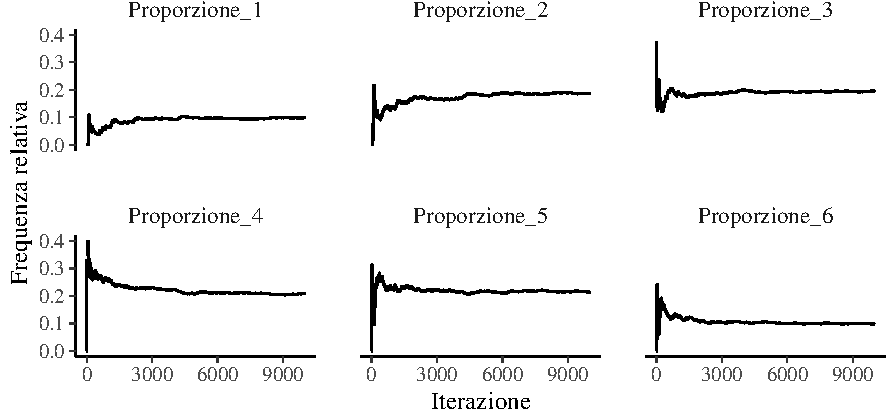
\includegraphics{035_approx_posterior_files/figure-latex/markovsim-1} 

}

\caption{Frequenze relative degli stati da 1 a 6 in funzione del numero di iterazioni per la simulazione di una catena di Markov.}\label{fig:markovsim}
\end{figure}

\hypertarget{campionamento-mediante-algoritmi-mcmc}{%
\subsection{Campionamento mediante algoritmi MCMC}\label{campionamento-mediante-algoritmi-mcmc}}

Il metodo di campionamento utilizzato dagli algoritmi Monte Carlo a catena di Markov (MCMC) crea una catena di Markov irriducibile e aperiodica, la cui distribuzione stazionaria equivale alla distribuzione a posteriori \(p(\theta \mid y)\). Un modo generale per ottenere una tale catena di Markov è quello di usare l'algoritmo di Metropolis. L'algoritmo di Metropolis è il primo algoritmo MCMC che è stato proposto, ed è applicabile ad una grande varietà di problemi inferenziali di tipo bayesiano. Tale algoritmo è stato in seguito sviluppato allo scopo di renderlo via via più efficiente. Lo presentiamo qui in una forma intuitiva.

\hypertarget{una-passeggiata-casuale-sui-numeri-naturali}{%
\subsection{Una passeggiata casuale sui numeri naturali}\label{una-passeggiata-casuale-sui-numeri-naturali}}

Per introdurre l'algoritmo di di Metropolis considereremo il campionamento da una distribuzione discreta.\footnote{Seguiamo qui la trattazione di \citet{albert2019probability}. Per una presentazione intuitiva dell'algoritmo di Metropolis, si vedano anche \citet{doing_bayesian_data_an}; \citet{McElreath_rethinking}.} Supponiamo di definire una distribuzione di probabilità discreta sugli interi \(1,\dots, K\). Scriviamo in \(\R\) la funzione \texttt{pd()} che assegna ai valori \(1,\dots, 8\) delle probabilità proporzionali a 5, 10, 4, 4, 20, 20, 12 e 5.

\begin{Shaded}
\begin{Highlighting}[]
\NormalTok{pd }\OtherTok{\textless{}{-}} \ControlFlowTok{function}\NormalTok{(x)\{}
\NormalTok{  values }\OtherTok{\textless{}{-}} \FunctionTok{c}\NormalTok{(}\DecValTok{5}\NormalTok{, }\DecValTok{10}\NormalTok{, }\DecValTok{4}\NormalTok{, }\DecValTok{4}\NormalTok{, }\DecValTok{20}\NormalTok{, }\DecValTok{20}\NormalTok{, }\DecValTok{12}\NormalTok{, }\DecValTok{5}\NormalTok{)}
  \FunctionTok{ifelse}\NormalTok{(}
\NormalTok{    x }\SpecialCharTok{\%in\%} \DecValTok{1}\SpecialCharTok{:}\FunctionTok{length}\NormalTok{(values),}
\NormalTok{    values[x] }\SpecialCharTok{/} \FunctionTok{sum}\NormalTok{(values),}
    \DecValTok{0}
\NormalTok{  )}
\NormalTok{\}}

\NormalTok{prob\_dist }\OtherTok{\textless{}{-}} \FunctionTok{tibble}\NormalTok{(}
  \AttributeTok{x =} \DecValTok{1}\SpecialCharTok{:}\DecValTok{8}\NormalTok{,}
  \AttributeTok{prob =} \FunctionTok{pd}\NormalTok{(}\DecValTok{1}\SpecialCharTok{:}\DecValTok{8}\NormalTok{)}
\NormalTok{)}
\end{Highlighting}
\end{Shaded}

\noindent
La figura \ref{fig:formetropolisdistr} illustra la distribuzione di probabilità che è stata generata.

\begin{Shaded}
\begin{Highlighting}[]
\NormalTok{x }\OtherTok{\textless{}{-}} \DecValTok{1}\SpecialCharTok{:}\DecValTok{8}
\NormalTok{prob\_dist }\SpecialCharTok{\%\textgreater{}\%}
  \FunctionTok{ggplot}\NormalTok{(}\FunctionTok{aes}\NormalTok{(}\AttributeTok{x =}\NormalTok{ x, }\AttributeTok{y =}\NormalTok{ prob)) }\SpecialCharTok{+}
  \FunctionTok{geom\_bar}\NormalTok{(}\AttributeTok{stat =} \StringTok{"identity"}\NormalTok{, }\AttributeTok{width =} \FloatTok{0.06}\NormalTok{) }\SpecialCharTok{+}
  \FunctionTok{scale\_x\_continuous}\NormalTok{(}\StringTok{"x"}\NormalTok{, }\AttributeTok{labels =} \FunctionTok{as.character}\NormalTok{(x), }\AttributeTok{breaks =}\NormalTok{ x) }\SpecialCharTok{+}
  \FunctionTok{labs}\NormalTok{(}
    \AttributeTok{y =} \StringTok{"Probabilità"}\NormalTok{,}
    \AttributeTok{x =} \StringTok{"X"}
\NormalTok{  )}
\end{Highlighting}
\end{Shaded}

\begin{figure}

{\centering 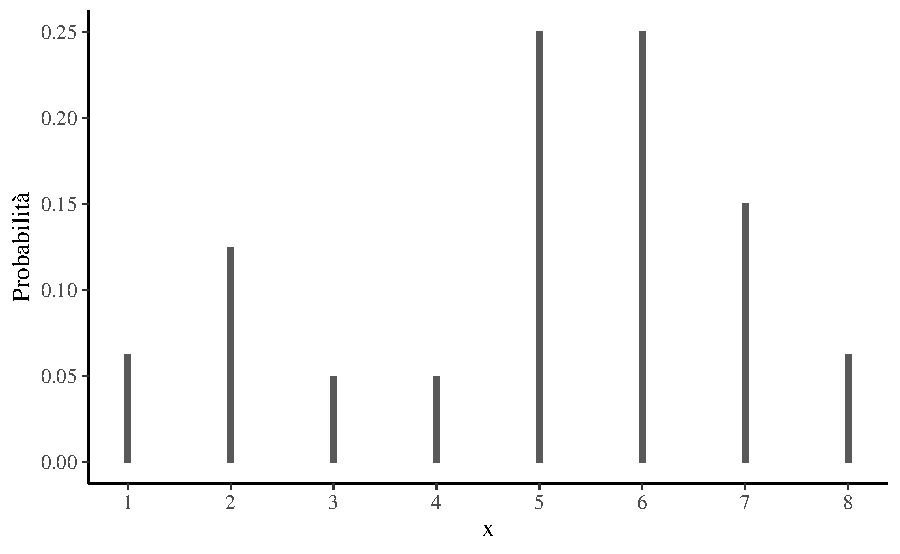
\includegraphics{035_approx_posterior_files/figure-latex/formetropolisdistr-1} 

}

\caption{Distribuzione di massa di probabilità per una variabile casuale avente valori 1, 2, ..., 8.}\label{fig:formetropolisdistr}
\end{figure}

\noindent
L'algoritmo di Metropolis corrisponde alla seguente passeggiata casuale.

\begin{enumerate}
\def\labelenumi{\arabic{enumi}.}
\item
  L'algoritmo inizia con un valore iniziale qualsiasi da 1 a \(K=8\) della variabile casuale.
\item
  Per simulare il valore successivo della sequenza, lanciamo una moneta equilibrata. Se esce testa, consideriamo come valore candidato il valore immediatamente precedente al valore corrente nella sequenza \(1, \dots, 8\); se esce croce, il valore candidato sarà il valore immediatamente successivo al valore corrente nella sequenza.
\item
  Calcoliamo il rapporto tra la probabilità del valore candidato e la probabilità del valore corrente:
\end{enumerate}

\[
R = \frac{pd(\text{valore candidato})}{pd(\text{valore corrente})}.
\]
4. Estraiamo un numero a caso \(\in [0, 1]\). Se tale valore è minore di \(R\) accettiamo il valore candidato come valore successivo della catena markoviana; altrimenti il valore successivo della catena rimane il valore corrente.

\bigskip

I passi da 1 a 4 definiscono una catena di Markov irriducibile e aperiodica sui valori di stato \(\{1, 2,\dots, 8\}\), dove il passo 1 fornisce il valore iniziale della catena e i passi da 2 a 4 definiscono la matrice di transizione \(P\). Un modo di campionare da una distribuzione di massa di probabilità \texttt{pd} consiste nell'iniziare da una posizione qualsiasi e eseguire una passeggiata casuale costituita da un grande numero di passi, ripetendo le fasi 2, 3 e 4 dell'algoritmo di Metropolis. Dopo un grande numero di passi, la distribuzione dei valori della catena markoviana approssimerà la distribuzione di probabilità \texttt{pd}.

La funzione \texttt{random\_walk()} implementa l'algoritmo di Metropolis. Tale funzione richiede in input la distribuzione di probabilità \texttt{pd}, la posizione di partenza \texttt{start} e il numero di passi dell'algoritmo \texttt{num\_steps}.

\begin{Shaded}
\begin{Highlighting}[]
\NormalTok{random\_walk }\OtherTok{\textless{}{-}} \ControlFlowTok{function}\NormalTok{(pd, start, num\_steps)\{}
\NormalTok{  y }\OtherTok{\textless{}{-}} \FunctionTok{rep}\NormalTok{(}\DecValTok{0}\NormalTok{, num\_steps)}
\NormalTok{  current }\OtherTok{\textless{}{-}}\NormalTok{ start}
  \ControlFlowTok{for}\NormalTok{ (j }\ControlFlowTok{in} \DecValTok{1}\SpecialCharTok{:}\NormalTok{num\_steps)\{}
\NormalTok{    candidate }\OtherTok{\textless{}{-}}\NormalTok{ current }\SpecialCharTok{+} \FunctionTok{sample}\NormalTok{(}\FunctionTok{c}\NormalTok{(}\SpecialCharTok{{-}}\DecValTok{1}\NormalTok{, }\DecValTok{1}\NormalTok{), }\DecValTok{1}\NormalTok{)}
\NormalTok{    prob }\OtherTok{\textless{}{-}} \FunctionTok{pd}\NormalTok{(candidate) }\SpecialCharTok{/} \FunctionTok{pd}\NormalTok{(current)}
    \ControlFlowTok{if}\NormalTok{ (}\FunctionTok{runif}\NormalTok{(}\DecValTok{1}\NormalTok{) }\SpecialCharTok{\textless{}}\NormalTok{ prob)}
\NormalTok{      current }\OtherTok{\textless{}{-}}\NormalTok{ candidate}
\NormalTok{    y[j] }\OtherTok{\textless{}{-}}\NormalTok{ current}
\NormalTok{  \}}
  \FunctionTok{return}\NormalTok{(y)}
\NormalTok{\}}
\end{Highlighting}
\end{Shaded}

\noindent
Di seguito, implementiamo l'algoritmo di Metropolis utilizzando, quale valore iniziale, \(X=4\). Ripetiamo la simulazione 10,000 volte.

\begin{Shaded}
\begin{Highlighting}[]
\NormalTok{out }\OtherTok{\textless{}{-}} \FunctionTok{random\_walk}\NormalTok{(pd, }\DecValTok{4}\NormalTok{, }\FloatTok{1e4}\NormalTok{)}

\NormalTok{S }\OtherTok{\textless{}{-}} \FunctionTok{tibble}\NormalTok{(out) }\SpecialCharTok{\%\textgreater{}\%}
  \FunctionTok{group\_by}\NormalTok{(out) }\SpecialCharTok{\%\textgreater{}\%}
  \FunctionTok{summarize}\NormalTok{(}
    \AttributeTok{N =} \FunctionTok{n}\NormalTok{(),}
    \AttributeTok{Prob =}\NormalTok{ N }\SpecialCharTok{/} \DecValTok{10000}
\NormalTok{  )}

\NormalTok{prob\_dist2 }\OtherTok{\textless{}{-}} \FunctionTok{rbind}\NormalTok{(}
\NormalTok{  prob\_dist,}
  \FunctionTok{tibble}\NormalTok{(}
    \AttributeTok{x =}\NormalTok{ S}\SpecialCharTok{$}\NormalTok{out,}
    \AttributeTok{prob =}\NormalTok{ S}\SpecialCharTok{$}\NormalTok{Prob}
\NormalTok{    )}
\NormalTok{  )}
\NormalTok{prob\_dist2}\SpecialCharTok{$}\NormalTok{Type }\OtherTok{\textless{}{-}} \FunctionTok{rep}\NormalTok{(}
  \FunctionTok{c}\NormalTok{(}\StringTok{"Prob. corrette"}\NormalTok{, }\StringTok{"Prob. simulate"}\NormalTok{), }
  \AttributeTok{each =} \DecValTok{8}
\NormalTok{  )}
\end{Highlighting}
\end{Shaded}

\begin{Shaded}
\begin{Highlighting}[]
\NormalTok{x }\OtherTok{\textless{}{-}} \DecValTok{1}\SpecialCharTok{:}\DecValTok{8}
\NormalTok{prob\_dist2 }\SpecialCharTok{\%\textgreater{}\%}
  \FunctionTok{ggplot}\NormalTok{(}\FunctionTok{aes}\NormalTok{(}\AttributeTok{x =}\NormalTok{ x, }\AttributeTok{y =}\NormalTok{ prob, }\AttributeTok{fill =}\NormalTok{ Type)) }\SpecialCharTok{+}
  \FunctionTok{geom\_bar}\NormalTok{(}\AttributeTok{stat =} \StringTok{"identity"}\NormalTok{, }\AttributeTok{width =} \FloatTok{0.1}\NormalTok{, }\AttributeTok{position =} \FunctionTok{position\_dodge}\NormalTok{(}\FloatTok{0.3}\NormalTok{)) }\SpecialCharTok{+}
  \FunctionTok{scale\_x\_continuous}\NormalTok{(}\StringTok{"x"}\NormalTok{, }\AttributeTok{labels =} \FunctionTok{as.character}\NormalTok{(x), }\AttributeTok{breaks =}\NormalTok{ x) }\SpecialCharTok{+}
  \FunctionTok{scale\_fill\_manual}\NormalTok{(}\AttributeTok{values =} \FunctionTok{c}\NormalTok{(}\StringTok{"black"}\NormalTok{, }\StringTok{"gray80"}\NormalTok{)) }\SpecialCharTok{+}
  \FunctionTok{theme}\NormalTok{(}\AttributeTok{legend.title =} \FunctionTok{element\_blank}\NormalTok{()) }\SpecialCharTok{+}
  \FunctionTok{labs}\NormalTok{(}
    \AttributeTok{y =} \StringTok{"Probabilità"}\NormalTok{,}
    \AttributeTok{x =} \StringTok{"X"}
\NormalTok{  )}
\end{Highlighting}
\end{Shaded}

\begin{figure}

{\centering 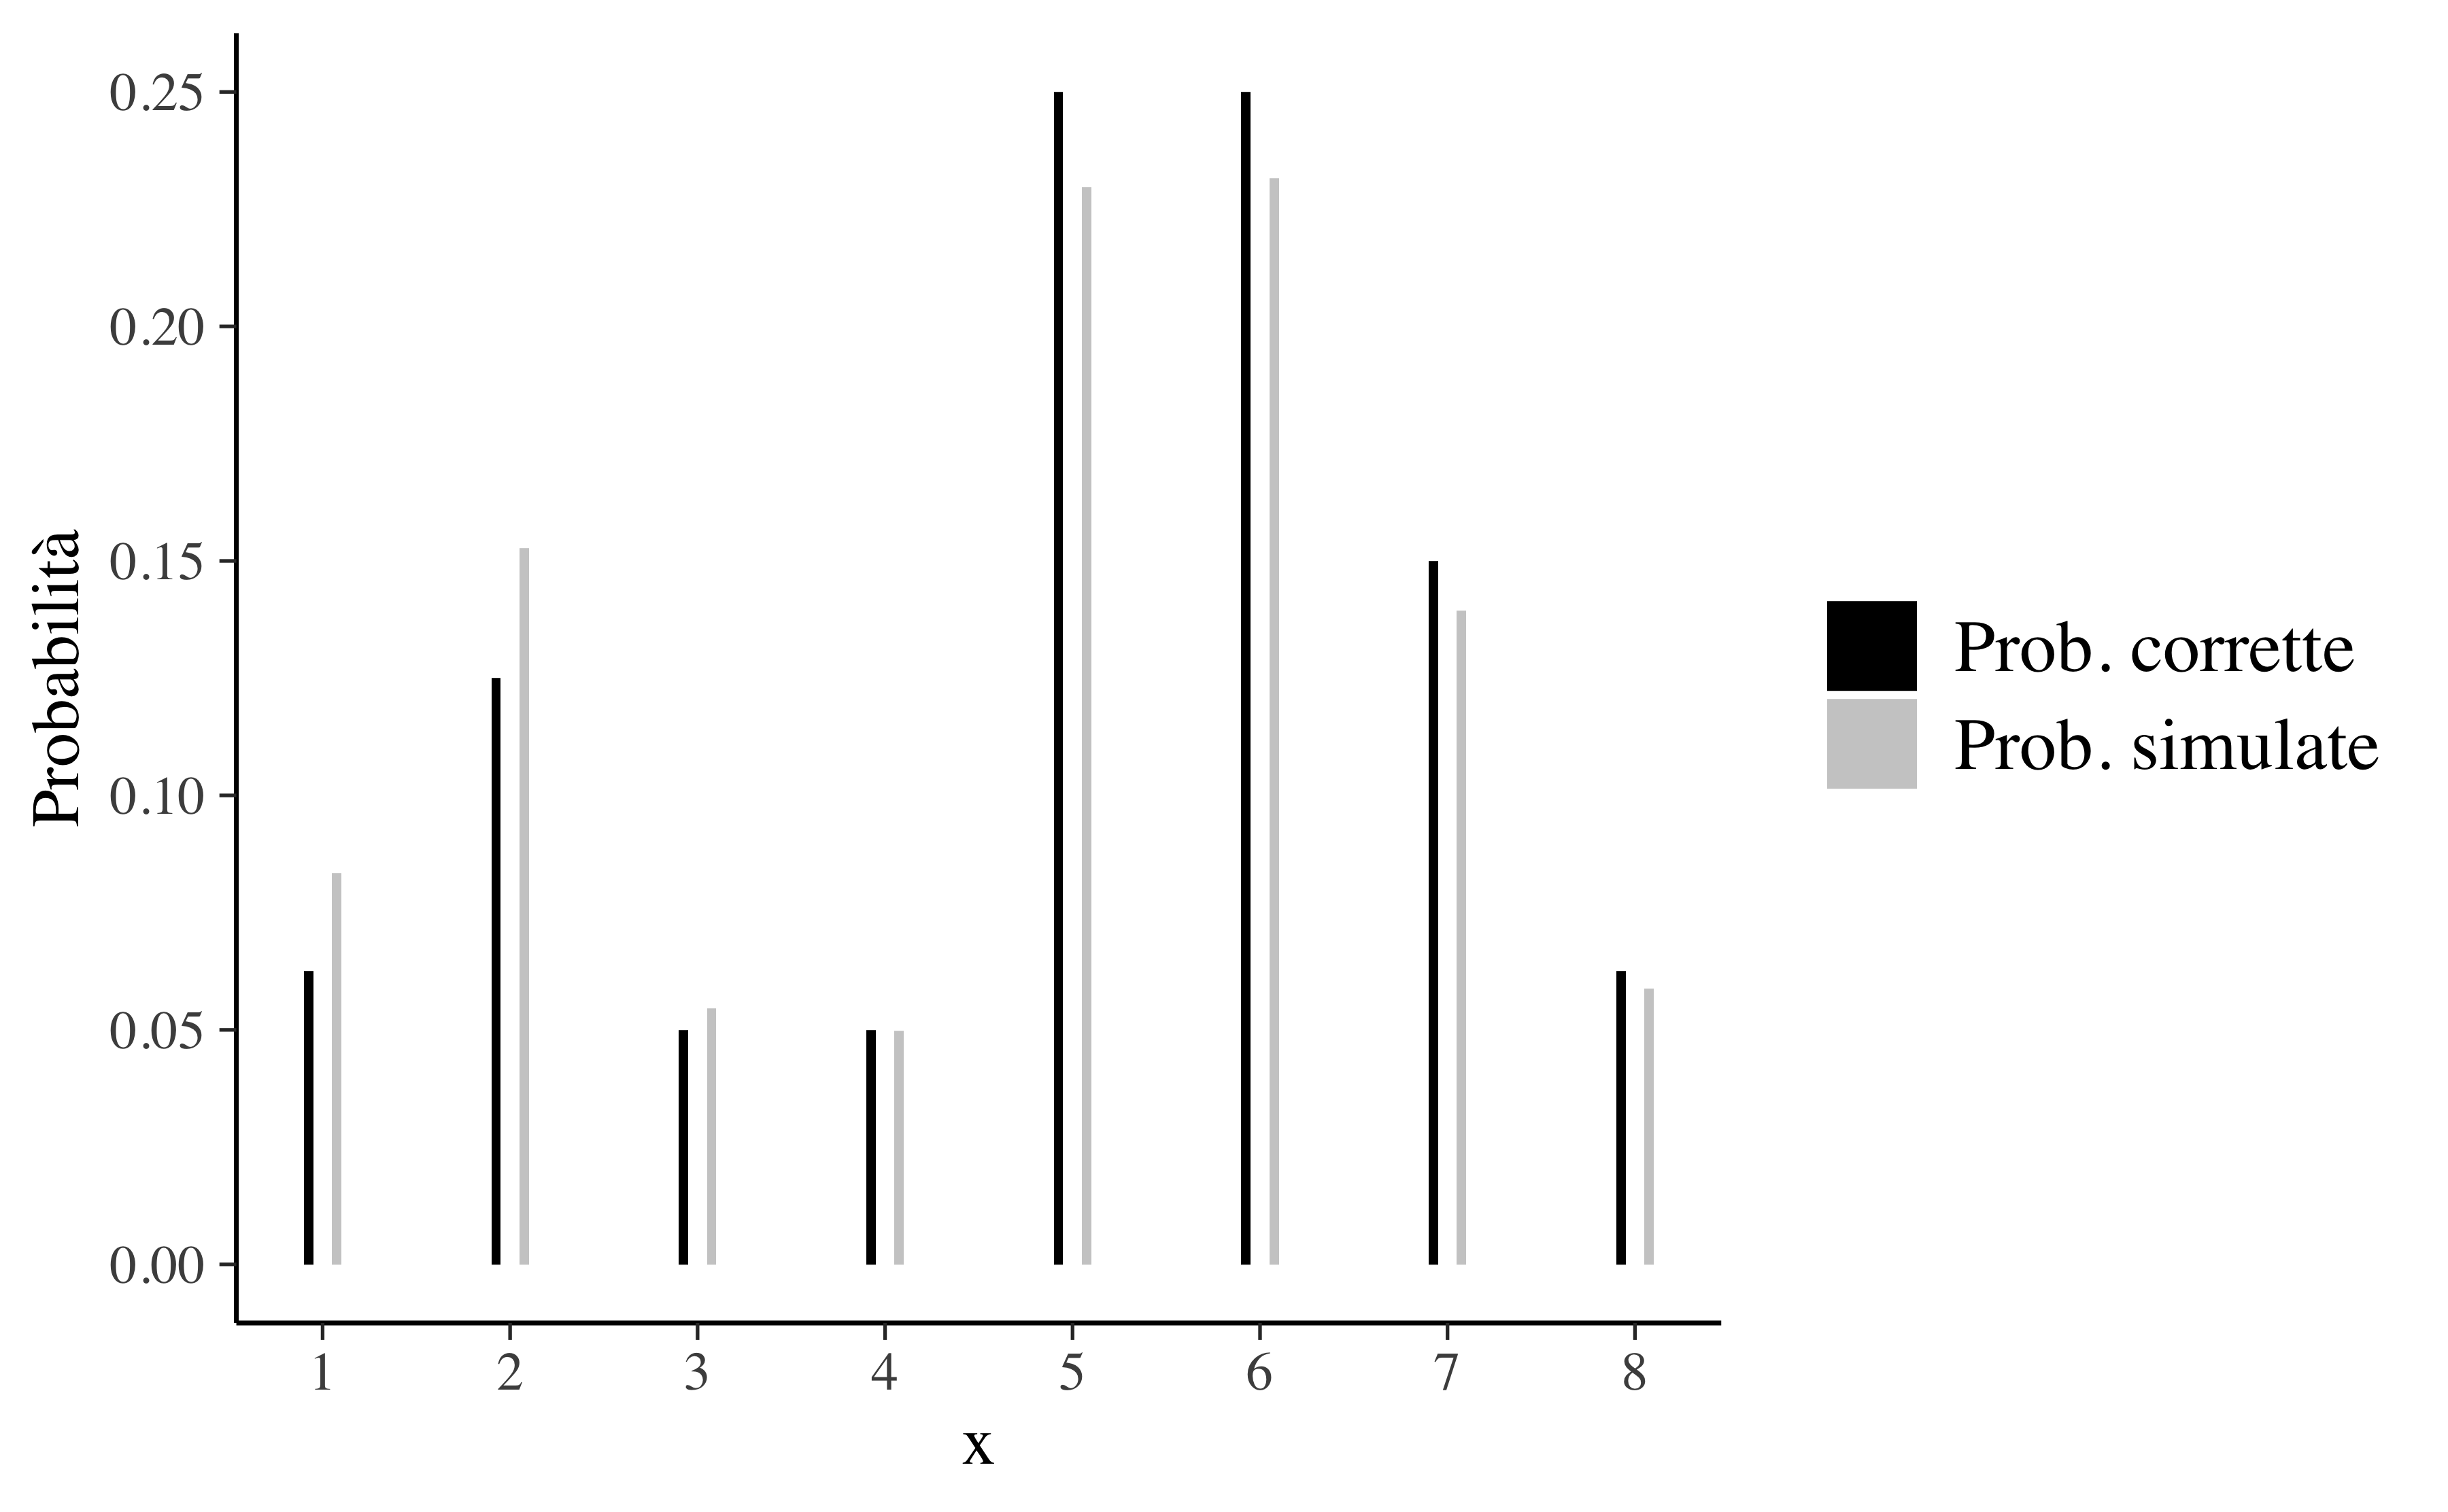
\includegraphics{035_approx_posterior_files/figure-latex/metropolishistogramsim-1} 

}

\caption{L'istogramma confronta i valori prodotti dall'algoritmo di Metropolis con i corretti valori della distribuzione di massa di probabilità.}\label{fig:metropolishistogramsim}
\end{figure}

\noindent
La figura \ref{fig:metropolishistogramsim} confronta l'istogramma dei valori simulati dalla passeggiata casuale con l'effettiva distribuzione di probabilità \texttt{pd}. Si noti la somiglianza tra le due distribuzioni.

\hypertarget{lalgoritmo-di-metropolis}{%
\subsection{L'algoritmo di Metropolis}\label{lalgoritmo-di-metropolis}}

Vediamo ora come l'algoritmo di Metropolis possa venire usato per generare una catena di Markov irriducibile e aperiodica per la quale la distribuzione stazionaria è uguale alla distribuzione a posteriori di interesse.\footnote{Una illustrazione visiva di come si svolge il processo di ``esplorazione'' dell'algoritmo di Metropolis è fornita in questo \href{https://elevanth.org/blog/2017/11/28/build-a-better-markov-chain/}{post}.}

In termini generali, l'algoritmo di Metropolis include due fasi.

\begin{itemize}
\tightlist
\item
  \emph{Fase 1} La selezione di un valore candidato \(\theta'\) del parametro mediante il campionamento da una distribuzione proposta.
\item
  \emph{Fase 2} La decisione tra la possibilità di accettare il valore candidato
  \[
  \theta^{(m+1)} = \theta'
  \]
  \noindent
  o di mantenere il valore corrente
  \[
  \theta^{(m+1)} = \theta
  \]
  \noindent
  sulla base del seguente criterio:

  \begin{itemize}
  \tightlist
  \item
    se \(\mathcal{L}(\theta' \mid y)p(\theta') > \mathcal{L}(\theta \mid y)p(\theta)\) il valore candidato viene sempre accettato;
  \item
    altrimenti il valore candidato viene accettato solo in una certa proporzione di casi.
  \end{itemize}
\end{itemize}

Esaminiamo ora nei dettagli il funzionamento dell'algoritmo di Metropolis.

\begin{enumerate}
\def\labelenumi{(\alph{enumi})}
\item
  Si inizia con un punto arbitrario \(\theta^{(1)}\), quindi il primo valore della catena di Markov \(\theta^{(1)}\) può corrispondere semplicemente ad un valore a caso tra i valori possibili del parametro.
\item
  Per ogni passo successivo della catena, \(m + 1\), si campiona un valore candidato \(\theta'\) da una distribuzione proposta: \(\theta' \sim \Pi(\theta)\). La distribuzione proposta può essere qualunque distribuzione, anche se, idealmente, è meglio che sia simile alla distribuzione a posteriori. In pratica la distribuzione a posteriori è sconosciuta e quindi il valore \(\theta'\) viene campionato da una qualche distribuzione simmetrica centrata sul valore corrente \(\theta^{(m)}\) del parametro. Nell'esempio che verrà discusso qui sotto, useremo la distribuzione Normale. Tale distribuzione sarà centrata sul valore corrente della catena e avrà una appropriata deviazione standard: \(\theta' \sim \mathcal{N}(\theta^{(m)}, \sigma)\). In pratica, questo significa che, se \(\sigma\) è piccola, il valore candidato \(\theta'\) sarà simile al valore corrente \(\theta^{(m)}\).
\item
  Una volta generato il valore candidato \(\theta'\) si calcola il rapporto tra la densità della distribuzione a posteriori non normalizzata nel punto \(\theta'\) {[}ovvero, il prodotto tra la verosimiglianza \(\mathcal{L}(y \mid \theta')\) nel punto \(\theta'\) e la distribuzione a priori nel punto \(\theta'\){]} e la densità della distribuzione a posteriori non normalizzata nel punto \(\theta^{(m)}\) {[}ovvero, il prodotto tra la verosimiglianza \(\mathcal{L}(y \mid \theta^{(m)})\) nel punto \(\theta^{(m)}\) e la distribuzione a priori nel punto \(\theta^{(m)}\){]}:
\end{enumerate}

\begin{equation}
\alpha = \frac{p(y \mid \theta') p(\theta')}{p(y \mid \theta^{(m)}) p(\theta^{(m)})}.
\label{eq:ratio-metropolis}
\end{equation}

\noindent
Si noti che, essendo un rapporto, la \eqref{eq:ratio-metropolis} cancella la costante di normalizzazione.

\begin{enumerate}
\def\labelenumi{(\alph{enumi})}
\setcounter{enumi}{3}
\item
  Il rapporto \(\alpha\) viene utilizzato per decidere se accettare il valore candidato \(\theta'\), oppure se campionare un diverso candidato. Possiamo pensare al rapporto \(\alpha\) come alla risposta alla seguente domanda: alla luce dei dati, è più plausibile il valore candidato del parametro o il valore corrente? Se \(\alpha\) è maggiore di 1 ciò significa che il valore candidato è più plausibile del valore corrente; in tali circostanze il valore candidato viene sempre accettato. Altrimenti, si decide di accettare il valore candidato con una probabilità minore di 1, ovvero non sempre, ma soltanto con una probabilità uguale ad \(\alpha\). Se \(\alpha\) è uguale a 0.10, ad esempio, questo significa che la plausibilità a posteriori del valore candidato è 10 volte più piccola della plausibilità a posteriori del valore corrente. Dunque, il valore candidato verrà accettato solo nel 10\% dei casi. Come conseguenza di questa strategia di scelta, l'algoritmo di Metropolis ottiene un campione casuale dalla distribuzione a posteriori, dato che la probabilità di accettare il valore candidato è proporzionale alla densità del candidato nella distribuzione a posteriori. Dal punto di vista algoritmico, la procedura descritta sopra viene implementata confrontando il rapporto \(\alpha\) con un valore casuale estratto da una distribuzione uniforme \(\mbox{Unif}(0, 1)\). Se \(\alpha > u \sim \mbox{Unif}(0, 1)\) allora il punto candidato \(\theta'\) viene accettato e la catena si muove in quella nuova posizione, ovvero \(\theta^{(m+1)} = \theta'^{(m+1)}\). Altrimenti \(\theta^{(m+1)} = \theta^{(m)}\) e si campiona un nuovo valore candidato \(\theta'\).
\item
  Il passaggio finale dell'algoritmo calcola l'\emph{accettanza} in una specifica esecuzione dell'algoritmo, ovvero la proporzione dei valori candidati \(\theta'\) che sono stati accettati come valori successivi nella sequenza.
\end{enumerate}

L'algoritmo di Metropolis prende come input il numero \(M\) di passi da simulare, la deviazione standard \(\sigma\) della distribuzione proposta e la densità a priori, e ritorna come output la sequenza \(\theta^{(1)}, \theta^{(2)}, \dots, \theta^{(M)}\). La chiave del successo dell'algoritmo di Metropolis è il numero di passi fino a che la catena approssima la stazionarietà. Tipicamente i primi da 1000 a 5000 elementi sono scartati. Dopo un certo periodo \(k\) (detto di \emph{burn-in}), la catena di Markov converge ad una variabile casuale che è distribuita secondo la distribuzione a posteriori. In altre parole, i campioni del vettore \(\left(\theta^{(k+1)}, \theta^{(k+2)}, \dots, \theta^{(M)}\right)\) diventano campioni di \(p(\theta \mid y)\).

\hypertarget{una-applicazione-concreta}{%
\subsection{Una applicazione concreta}\label{una-applicazione-concreta}}

Per fare un esempio concreto, consideriamo nuovamente i 30 pazienti esaminati da \citet{zetschefuture2019} e discussi nel Paragrafo \ref{es-pratico-zetsche}. Di essi, 23 hanno manifestato aspettative distorte negativamente sul loro stato d'animo futuro. Utilizzando l'algoritmo di Metropolis, ci poniamo il problema di ottenere la stima a posteriori di \(\theta\) (probabilità di manifestare un'aspettativa distorta negativamente), dati 23 ``successi'' in 30 prove. Verrà imposta a \(\theta\) la stessa distribuzione a priori usata nel Paragrafo \ref{es-depression-beta-2-10}.

\hypertarget{verosimiglianza}{%
\subsubsection{Verosimiglianza}\label{verosimiglianza}}

Per calcolare la funzione di verosimiglianza per i 30 valori di \citet{zetschefuture2019} useremo la funzione \texttt{likelihood()}:

\begin{Shaded}
\begin{Highlighting}[]
\NormalTok{x }\OtherTok{\textless{}{-}} \DecValTok{23}
\NormalTok{N }\OtherTok{\textless{}{-}} \DecValTok{30}
\NormalTok{param }\OtherTok{\textless{}{-}} \FunctionTok{seq}\NormalTok{(}\DecValTok{0}\NormalTok{, }\DecValTok{1}\NormalTok{, }\AttributeTok{length.out =} \DecValTok{100}\NormalTok{)}

\NormalTok{likelihood }\OtherTok{\textless{}{-}} \ControlFlowTok{function}\NormalTok{(param, }\AttributeTok{x =} \DecValTok{23}\NormalTok{, }\AttributeTok{N =} \DecValTok{30}\NormalTok{) \{}
  \FunctionTok{dbinom}\NormalTok{(x, N, param)}
\NormalTok{\}}

\FunctionTok{tibble}\NormalTok{(}
  \AttributeTok{x =}\NormalTok{ param, }
  \AttributeTok{y =} \FunctionTok{likelihood}\NormalTok{(param)}
\NormalTok{) }\SpecialCharTok{\%\textgreater{}\%}
  \FunctionTok{ggplot}\NormalTok{(}\FunctionTok{aes}\NormalTok{(x, y)) }\SpecialCharTok{+}
  \FunctionTok{geom\_line}\NormalTok{() }\SpecialCharTok{+}
  \FunctionTok{labs}\NormalTok{(}
    \AttributeTok{x =} \FunctionTok{expression}\NormalTok{(theta),}
    \AttributeTok{y =} \StringTok{"Verosimiglianza"}
\NormalTok{  )}
\end{Highlighting}
\end{Shaded}

\begin{center}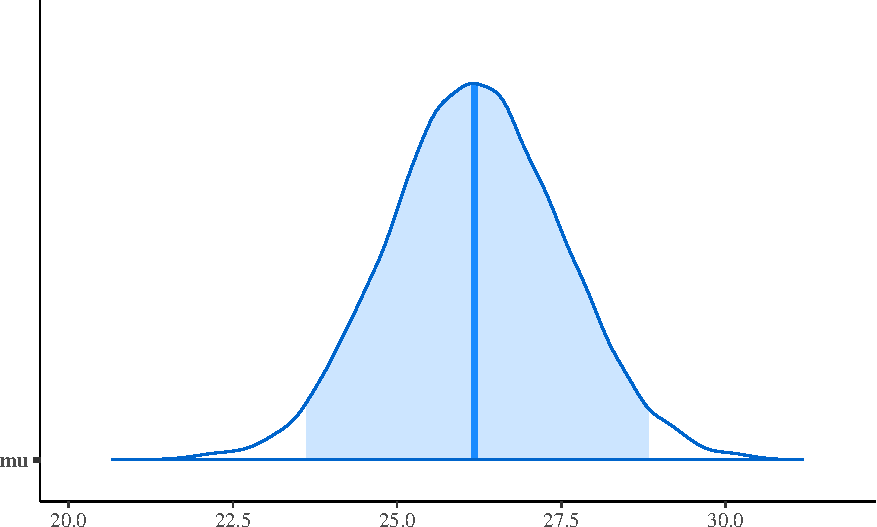
\includegraphics{035_approx_posterior_files/figure-latex/unnamed-chunk-19-1} \end{center}

\noindent
La funzione \texttt{likelihood()} ritorna l'ordinata della verosimiglianza binomiale per ciascun valore del vettore \texttt{param} in input.

\hypertarget{distribuzione-a-priori}{%
\subsubsection{Distribuzione a priori}\label{distribuzione-a-priori}}

Quale distribuzione a priori utilizzeremo una \(\mbox{Beta}(2, 10)\) implementata nella funzione \texttt{prior()}:

\begin{Shaded}
\begin{Highlighting}[]
\NormalTok{prior }\OtherTok{\textless{}{-}} \ControlFlowTok{function}\NormalTok{(param, }\AttributeTok{alpha =} \DecValTok{2}\NormalTok{, }\AttributeTok{beta =} \DecValTok{10}\NormalTok{) \{}
\NormalTok{  param\_vals }\OtherTok{\textless{}{-}} \FunctionTok{seq}\NormalTok{(}\DecValTok{0}\NormalTok{, }\DecValTok{1}\NormalTok{, }\AttributeTok{length.out =} \DecValTok{100}\NormalTok{)}
  \FunctionTok{dbeta}\NormalTok{(param, alpha, beta) }\CommentTok{\# / sum(dbeta(param\_vals, alpha, beta))}
\NormalTok{\}}

\FunctionTok{tibble}\NormalTok{(}
  \AttributeTok{x =}\NormalTok{ param, }
  \AttributeTok{y =} \FunctionTok{prior}\NormalTok{(param)}
\NormalTok{) }\SpecialCharTok{\%\textgreater{}\%}
  \FunctionTok{ggplot}\NormalTok{(}\FunctionTok{aes}\NormalTok{(x, y)) }\SpecialCharTok{+}
  \FunctionTok{geom\_line}\NormalTok{() }\SpecialCharTok{+}
  \FunctionTok{labs}\NormalTok{(}
    \AttributeTok{x =} \FunctionTok{expression}\NormalTok{(theta),}
    \AttributeTok{y =} \StringTok{"Densità"}
\NormalTok{  )}
\end{Highlighting}
\end{Shaded}

\begin{center}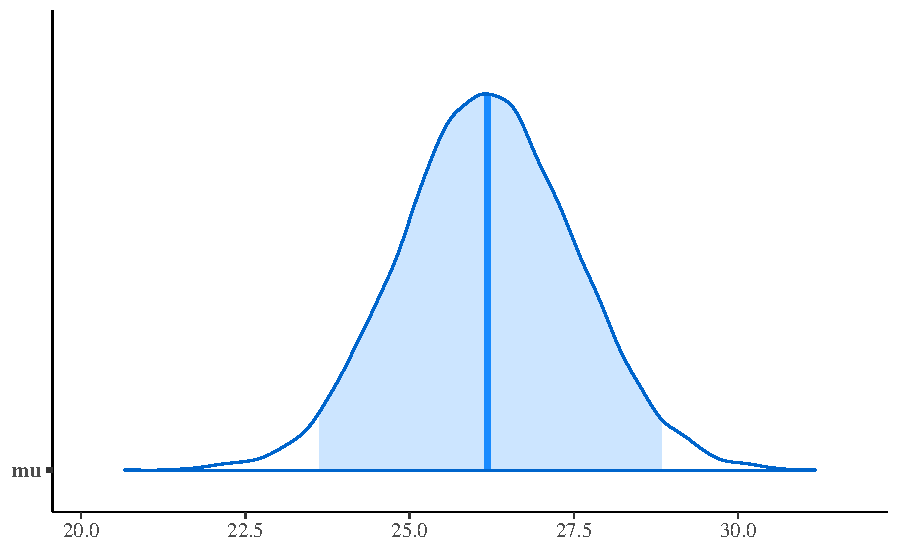
\includegraphics{035_approx_posterior_files/figure-latex/unnamed-chunk-20-1} \end{center}

\hypertarget{distribuzione-a-posteriori}{%
\subsubsection{Distribuzione a posteriori}\label{distribuzione-a-posteriori}}

La funzione a posteriori è data dal prodotto della densità a priori e della verosimiglianza ed è implementata nella funzione \texttt{posterior()}:

\begin{Shaded}
\begin{Highlighting}[]
\NormalTok{posterior }\OtherTok{\textless{}{-}} \ControlFlowTok{function}\NormalTok{(param) \{}
  \FunctionTok{likelihood}\NormalTok{(param) }\SpecialCharTok{*} \FunctionTok{prior}\NormalTok{(param)}
\NormalTok{\}}

\FunctionTok{tibble}\NormalTok{(}
  \AttributeTok{x =}\NormalTok{ param, }
  \AttributeTok{y =} \FunctionTok{posterior}\NormalTok{(param)}
\NormalTok{) }\SpecialCharTok{\%\textgreater{}\%}
  \FunctionTok{ggplot}\NormalTok{(}\FunctionTok{aes}\NormalTok{(x, y)) }\SpecialCharTok{+}
  \FunctionTok{geom\_line}\NormalTok{() }\SpecialCharTok{+}
  \FunctionTok{labs}\NormalTok{(}
    \AttributeTok{x =} \FunctionTok{expression}\NormalTok{(theta),}
    \AttributeTok{y =} \StringTok{"Densità"}
\NormalTok{  )}
\end{Highlighting}
\end{Shaded}

\begin{center}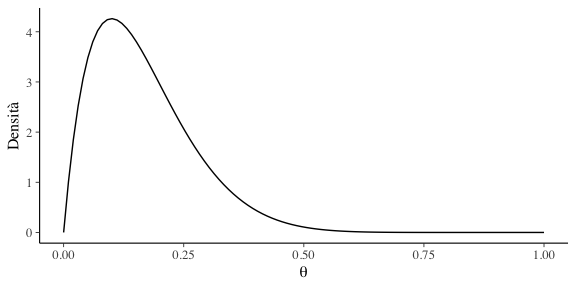
\includegraphics{035_approx_posterior_files/figure-latex/unnamed-chunk-21-1} \end{center}

Il risultato della figura precedente è stato ottenuto con il metodo basato su griglia. Vogliamo ora replicare tale risultato usando l'algoritmo di Metropolis. La figura indica che la media a posteriori è pari a circa 0.6. Questo è il valore a posteriori più verosimile per il parametro \(\theta\) alla luce dei dati osservati se assumiamo una distribuzione a priori \(\mbox{Beta}(2, 10)\). Ci poniamo ora il problema di replicare tale risultato usando l'algoritmo di Metropolis.

\hypertarget{implementazione}{%
\subsubsection{Implementazione}\label{implementazione}}

Per implementare l'algoritmo di Metropolis utilizzeremo una distribuzione proposta Normale. Il valore candidato sarà dunque un valore selezionato a caso da una Normale di parametri \(\mu\) uguale al valore corrente nella catena e \(\sigma = 0.9\). In questo esempio, la deviazione standard \(\sigma\) è stata scelta empiricamente in modo tale da ottenere una accettanza adeguata. L'accettanza ottimale è di circa 0.20 e 0.30 --- se l'accettanza è troppo grande, l'algoritmo esplora uno spazio troppo ristretto della distribuzione a posteriori.\footnote{L'accettanza dipende dalla distribuzione proposta: in generale, tanto più la distribuzione proposta è simile alla distribuzione target, tanto più alta diventa l'accettanza.}

\begin{Shaded}
\begin{Highlighting}[]
\NormalTok{proposal\_distribution }\OtherTok{\textless{}{-}} \ControlFlowTok{function}\NormalTok{(param) \{}
  \ControlFlowTok{while}\NormalTok{(}\DecValTok{1}\NormalTok{) \{}
\NormalTok{    res }\OtherTok{=} \FunctionTok{rnorm}\NormalTok{(}\DecValTok{1}\NormalTok{, }\AttributeTok{mean =}\NormalTok{ param, }\AttributeTok{sd =} \FloatTok{0.9}\NormalTok{)}
    \ControlFlowTok{if}\NormalTok{ (res }\SpecialCharTok{\textgreater{}} \DecValTok{0} \SpecialCharTok{\&}\NormalTok{ res }\SpecialCharTok{\textless{}} \DecValTok{1}\NormalTok{)}
      \ControlFlowTok{break}
\NormalTok{  \}}
\NormalTok{  res}
\NormalTok{\}}
\end{Highlighting}
\end{Shaded}

\noindent 
Nella presente implementazione del campionamento dalla distribuzione proposta è stato inserito un controllo che impone al valore candidato di essere incluso nell'intervallo {[}0, 1{]}.\footnote{Si possono trovare implementazioni dell'algoritmo di Metropolis più eleganti di quella presentata qui. Lo scopo dell'esercizio è quello di illustrare la logica soggiacente all'algoritmo di Metropolis, non quello di proporre un'implementazione efficente dell'algoritmo.}

L'algoritmo di Metropolis viene implementato nella seguente funzione:

\begin{Shaded}
\begin{Highlighting}[]
\NormalTok{run\_metropolis\_MCMC }\OtherTok{\textless{}{-}} \ControlFlowTok{function}\NormalTok{(startvalue, iterations) \{}
\NormalTok{  chain }\OtherTok{\textless{}{-}} \FunctionTok{vector}\NormalTok{(}\AttributeTok{length =}\NormalTok{ iterations }\SpecialCharTok{+} \DecValTok{1}\NormalTok{)}
\NormalTok{  chain[}\DecValTok{1}\NormalTok{] }\OtherTok{\textless{}{-}}\NormalTok{ startvalue}
  \ControlFlowTok{for}\NormalTok{ (i }\ControlFlowTok{in} \DecValTok{1}\SpecialCharTok{:}\NormalTok{iterations) \{}
\NormalTok{    proposal }\OtherTok{\textless{}{-}} \FunctionTok{proposal\_distribution}\NormalTok{(chain[i])}
\NormalTok{    r }\OtherTok{\textless{}{-}} \FunctionTok{posterior}\NormalTok{(proposal) }\SpecialCharTok{/} \FunctionTok{posterior}\NormalTok{(chain[i])}
    \ControlFlowTok{if}\NormalTok{ (}\FunctionTok{runif}\NormalTok{(}\DecValTok{1}\NormalTok{) }\SpecialCharTok{\textless{}}\NormalTok{ r) \{}
\NormalTok{      chain[i }\SpecialCharTok{+} \DecValTok{1}\NormalTok{] }\OtherTok{\textless{}{-}}\NormalTok{ proposal}
\NormalTok{    \} }\ControlFlowTok{else}\NormalTok{ \{}
\NormalTok{      chain[i }\SpecialCharTok{+} \DecValTok{1}\NormalTok{] }\OtherTok{\textless{}{-}}\NormalTok{ chain[i]}
\NormalTok{    \}}
\NormalTok{  \}}
\NormalTok{  chain}
\NormalTok{\}}
\end{Highlighting}
\end{Shaded}

Avendo definito le funzioni precedenti, generiamo una catena di valori \(\theta\):

\begin{Shaded}
\begin{Highlighting}[]
\FunctionTok{set.seed}\NormalTok{(}\DecValTok{123}\NormalTok{)}
\NormalTok{startvalue }\OtherTok{\textless{}{-}} \FunctionTok{runif}\NormalTok{(}\DecValTok{1}\NormalTok{, }\DecValTok{0}\NormalTok{, }\DecValTok{1}\NormalTok{)}
\NormalTok{niter }\OtherTok{\textless{}{-}} \FloatTok{1e4}
\NormalTok{chain }\OtherTok{\textless{}{-}} \FunctionTok{run\_metropolis\_MCMC}\NormalTok{(startvalue, niter)}
\end{Highlighting}
\end{Shaded}

Mediante le istruzioni precedenti otteniamo una catena di Markov costituita da 10,001 valori. Escludiamo i primi 5,000 valori considerati come burn-in. Ci restano dunque con 5,001 valori che verranno considerati come un campione casuale estratto dalla distribuzione a posteriori \(p(\theta \mid y)\).

L'accettanza è pari a

\begin{Shaded}
\begin{Highlighting}[]
\NormalTok{burnIn }\OtherTok{\textless{}{-}}\NormalTok{ niter }\SpecialCharTok{/} \DecValTok{2}
\NormalTok{acceptance }\OtherTok{\textless{}{-}} \DecValTok{1} \SpecialCharTok{{-}} \FunctionTok{mean}\NormalTok{(}\FunctionTok{duplicated}\NormalTok{(chain[}\SpecialCharTok{{-}}\NormalTok{(}\DecValTok{1}\SpecialCharTok{:}\NormalTok{burnIn)]))}
\NormalTok{acceptance}
\CommentTok{\#\textgreater{} [1] 0.2511498}
\end{Highlighting}
\end{Shaded}

\noindent
il che conferma la bontà della deviazione standard (\(\sigma\) = 0.9) scelta per la distribuzione proposta.

A questo punto è facile ottenere una stima a posteriori del parametro \(\theta\). Per esempio, la stima della media a posteriori è:

\begin{Shaded}
\begin{Highlighting}[]
\FunctionTok{mean}\NormalTok{(chain[}\SpecialCharTok{{-}}\NormalTok{(}\DecValTok{1}\SpecialCharTok{:}\NormalTok{burnIn)])}
\CommentTok{\#\textgreater{} [1] 0.5921799}
\end{Highlighting}
\end{Shaded}

Una figura che mostra l'approssimazione di \(p(\theta \mid y)\) ottenuta con l'algoritmo di Metropolis, insieme ad un \emph{trace plot} dei valori della catena di Markov, viene prodotta usando le seguenti istruzioni:

\begin{Shaded}
\begin{Highlighting}[]
\NormalTok{p1 }\OtherTok{\textless{}{-}} \FunctionTok{tibble}\NormalTok{(}
  \AttributeTok{x =}\NormalTok{ chain[}\SpecialCharTok{{-}}\NormalTok{(}\DecValTok{1}\SpecialCharTok{:}\NormalTok{burnIn)]}
\NormalTok{  ) }\SpecialCharTok{\%\textgreater{}\%}
  \FunctionTok{ggplot}\NormalTok{(}\FunctionTok{aes}\NormalTok{(x)) }\SpecialCharTok{+}
  \FunctionTok{geom\_histogram}\NormalTok{() }\SpecialCharTok{+}
  \FunctionTok{labs}\NormalTok{(}
    \AttributeTok{x =} \FunctionTok{expression}\NormalTok{(theta),}
    \AttributeTok{y =} \StringTok{"Frequenza"}\NormalTok{,}
    \AttributeTok{title =} \StringTok{"Distribuzione a posteriori"}
\NormalTok{  ) }\SpecialCharTok{+}
  \FunctionTok{geom\_vline}\NormalTok{(}
    \AttributeTok{xintercept =} \FunctionTok{mean}\NormalTok{(chain[}\SpecialCharTok{{-}}\NormalTok{(}\DecValTok{1}\SpecialCharTok{:}\NormalTok{burnIn)])}
\NormalTok{  )}

\NormalTok{p2 }\OtherTok{\textless{}{-}} \FunctionTok{tibble}\NormalTok{(}
  \AttributeTok{x =} \DecValTok{1}\SpecialCharTok{:}\FunctionTok{length}\NormalTok{(chain[}\SpecialCharTok{{-}}\NormalTok{(}\DecValTok{1}\SpecialCharTok{:}\NormalTok{burnIn)]),}
  \AttributeTok{y =}\NormalTok{ chain[}\SpecialCharTok{{-}}\NormalTok{(}\DecValTok{1}\SpecialCharTok{:}\NormalTok{burnIn)]}
\NormalTok{  ) }\SpecialCharTok{\%\textgreater{}\%}
  \FunctionTok{ggplot}\NormalTok{(}\FunctionTok{aes}\NormalTok{(x, y)) }\SpecialCharTok{+}
  \FunctionTok{geom\_line}\NormalTok{() }\SpecialCharTok{+}
  \FunctionTok{labs}\NormalTok{(}
    \AttributeTok{x =} \StringTok{"Numero di passi"}\NormalTok{,}
    \AttributeTok{y =} \FunctionTok{expression}\NormalTok{(theta),}
    \AttributeTok{title =} \StringTok{"Valori della catena"}
\NormalTok{  ) }\SpecialCharTok{+}
  \FunctionTok{geom\_hline}\NormalTok{(}
    \AttributeTok{yintercept =} \FunctionTok{mean}\NormalTok{(chain[}\SpecialCharTok{{-}}\NormalTok{(}\DecValTok{1}\SpecialCharTok{:}\NormalTok{burnIn)]),}
    \AttributeTok{colour =} \StringTok{"gray"}
\NormalTok{  )}

\NormalTok{p1 }\SpecialCharTok{+}\NormalTok{ p2}
\end{Highlighting}
\end{Shaded}

\begin{figure}

{\centering 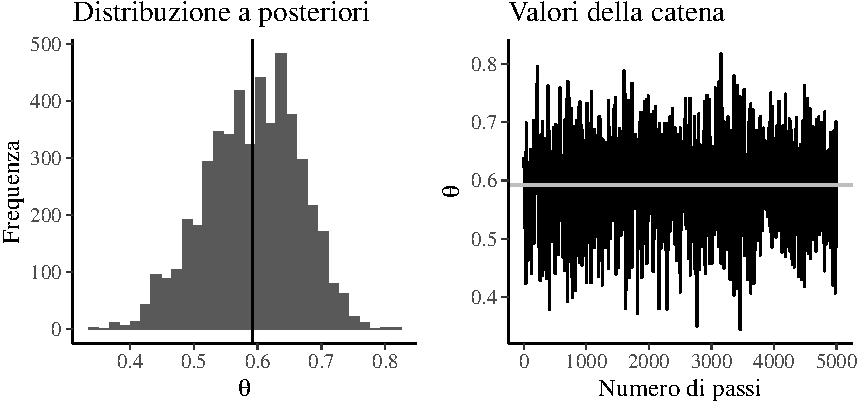
\includegraphics{035_approx_posterior_files/figure-latex/sim-markov-chain-zetsche-1} 

}

\caption{Sinistra. Stima della distribuzione a posteriori della probabilità di una aspettativa futura distorta negativamente per i dati di @zetschefuture2019. Destra. Trace plot dei valori della catena di Markov escludendo il periodo di burn-in.}\label{fig:sim-markov-chain-zetsche}
\end{figure}

\hypertarget{input}{%
\subsection{Input}\label{input}}

Negli esempi discussi in questo Capitolo abbiamo illustrato l'esecuzione di una singola catena in cui si parte un unico valore iniziale e si raccolgono i valori simulati da molte iterazioni. È possibile che i valori di una catena siano influenzati dalla scelta del valore iniziale. Quindi una raccomandazione generale è di eseguire l'algoritmo di Metropolis più volte utilizzando diversi valori di partenza. In questo caso, si avranno più catene di Markov. Confrontando le proprietà delle diverse catene si esplora la sensibilità dell'inferenza alla scelta del valore di partenza. I software MCMC consentono sempre all'utente di specificare diversi valori di partenza e di generare molteplici catene di Markov.

\hypertarget{stazionarietuxe0}{%
\section{Stazionarietà}\label{stazionarietuxe0}}

Un punto importante da verificare è se il campionatore ha raggiunto la sua distribuzione stazionaria. La convergenza di una catena di Markov alla distribuzione stazionaria viene detta ``mixing''.

\hypertarget{approx-post-autocor}{%
\subsection{Autocorrelazione}\label{approx-post-autocor}}

Informazioni sul ``mixing'' della catena di Markov sono fornite dall'autocorrelazione. L'autocorrelazione misura la correlazione tra i valori successivi di una catena di Markov. Il valore \(m\)-esimo della serie ordinata viene confrontato con un altro valore ritardato di una quantità \(k\) (dove \(k\) è l'entità del ritardo) per verificare quanto si correli al variare di \(k\). L'autocorrelazione di ordine 1 (\emph{lag 1}) misura la correlazione tra valori successivi della catena di Markow (cioè, la correlazione tra \(\theta^{(m)}\) e \(\theta^{(m-1)}\)); l'autocorrelazione di ordine 2 (\emph{lag 2}) misura la correlazione tra valori della catena di Markow separati da due ``passi'' (cioè, la correlazione tra \(\theta^{(m)}\) e \(\theta^{(m-2)}\)); e così via.

L'autocorrelazione di ordine \(k\) è data da \(\rho_k\) e può essere stimata come:

\begin{align}
\rho_k &= \frac{\Cov(\theta_m, \theta_{m+k})}{\Var(\theta_m)}\notag\\
&= \frac{\sum_{m=1}^{n-k}(\theta_m - \bar{\theta})(\theta_{m-k} - \bar{\theta})}{\sum_{m=1}^{n-k}(\theta_m - \bar{\theta})^2} \qquad\text{con }\quad \bar{\theta} = \frac{1}{n}\sum_{m=1}^{n}\theta_m.
\label{eq:autocor}
\end{align}

Per fare un esempio pratico, simuliamo dei dati autocorrelati con la funzione R \texttt{colorednoise::colored\_noise()}:

\begin{Shaded}
\begin{Highlighting}[]
\FunctionTok{suppressPackageStartupMessages}\NormalTok{(}\FunctionTok{library}\NormalTok{(}\StringTok{"colorednoise"}\NormalTok{))}
\FunctionTok{set.seed}\NormalTok{(}\DecValTok{34783859}\NormalTok{)}
\NormalTok{rednoise }\OtherTok{\textless{}{-}} \FunctionTok{colored\_noise}\NormalTok{(}
  \AttributeTok{timesteps =} \DecValTok{30}\NormalTok{, }\AttributeTok{mean =} \FloatTok{0.5}\NormalTok{, }\AttributeTok{sd =} \FloatTok{0.05}\NormalTok{, }\AttributeTok{phi =} \FloatTok{0.3}
\NormalTok{)}
\end{Highlighting}
\end{Shaded}

L'autocorrelazione di ordine 1 è semplicemente la correlazione tra ciascun elemento e quello successivo nella sequenza. Nell'esempio, il vettore \texttt{rednoise} è una sequenza temporale di 30 elementi. Il vettore \texttt{rednoise{[}-length(rednoise){]}} include gli elementi con gli indici da 1 a 29 nella sequenza originaria, mentre il vettore \texttt{rednoise{[}-1{]}} include gli elementi 2:30. Gli elementi delle coppie ordinate dei due vettori avranno dunque gli indici \((1, 2), (2, 3), \dots (29, 30)\) degli elementi della sequenza originaria. La correlazione di Pearson tra i vettori \texttt{rednoise{[}-length(rednoise){]}} e \texttt{rednoise{[}-1{]}} corrisponde dunque all'autocorrelazione di ordine 1 della serie temporale.

\begin{Shaded}
\begin{Highlighting}[]
\FunctionTok{cor}\NormalTok{(rednoise[}\SpecialCharTok{{-}}\FunctionTok{length}\NormalTok{(rednoise)], rednoise[}\SpecialCharTok{{-}}\DecValTok{1}\NormalTok{])}
\CommentTok{\#\textgreater{} [1] 0.3967366}
\end{Highlighting}
\end{Shaded}

Il Correlogramma è uno strumento grafico usato per la valutazione della tendenza di una catena di Markov nel tempo. Il correlogramma si costruisce a partire dall'autocorrelazione \(\rho_k\) di una catena di Markov in funzione del ritardo (\emph{lag}) \(k\) con cui l'autocorrelazione è calcolata: nel grafico ogni barretta verticale riporta il valore dell'autocorrelazione (sull'asse delle ordinate) in funzione del ritardo (sull'asse delle ascisse). In \(\R\), il correlogramma può essere prodotto con una chiamata a \texttt{acf()}:

\begin{Shaded}
\begin{Highlighting}[]
\FunctionTok{acf}\NormalTok{(rednoise)}
\end{Highlighting}
\end{Shaded}

\begin{center}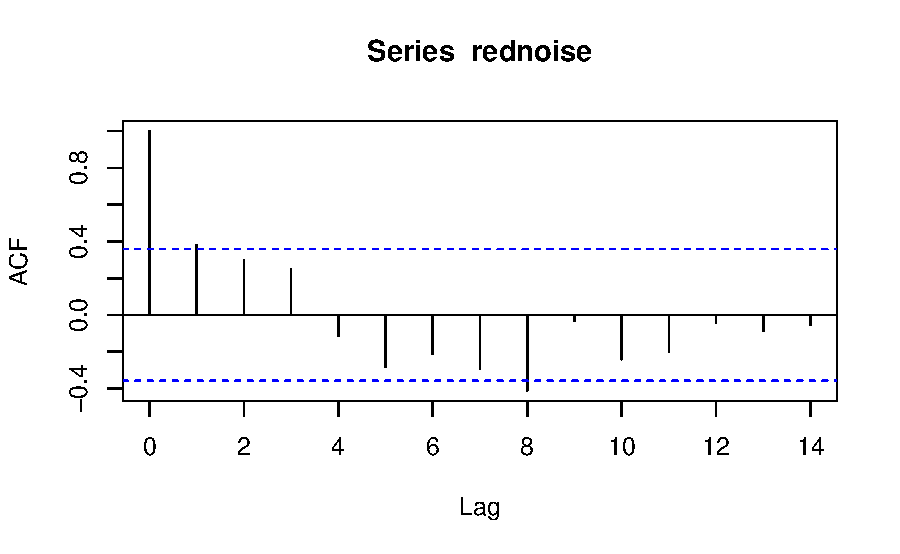
\includegraphics{035_approx_posterior_files/figure-latex/unnamed-chunk-29-1} \end{center}

Il correlogramma precedente mostra come l'autocorrelazione di ordine 1 sia circa pari a 0.4 e diminuisce per lag maggiori; per lag di 4, l'autocorrelazione diventa negativa e aumenta progressivamente fino ad un lag di 8; eccetera.

In situazioni ottimali l'autocorrelazione diminuisce rapidamente ed è effettivamente pari a 0 per piccoli lag. Ciò indica che i valori della catena di Markov che si trovano a più di soli pochi passi di distanza gli uni dagli altri non risultano associati tra loro, il che fornisce conferma del ``mixing'' della catena di Markov, ossia di convergenza alla distribuzione stazionaria.
Nelle analisi bayesiane, una delle strategie che consentono di ridurre l'autocorrelazione è quella di assottigliare l'output immagazzinando solo ogni \(m\)-esimo punto dopo il periodo di burn-in. Una tale strategia va sotto il nome di \emph{thinning}.

\hypertarget{test-di-convergenza}{%
\subsection{Test di convergenza}\label{test-di-convergenza}}

Un test di convergenza può essere svolto in maniera grafica mediante le tracce delle serie temporali (\emph{trace plot}), cioè il grafico dei valori simulati rispetto al numero di iterazioni. Se la catena è in uno stato stazionario le tracce mostrano assenza di periodicità nel tempo e ampiezza costante, senza tendenze visibili o andamenti degni di nota. Un esempio di \emph{trace plot} è fornito nella figura \ref{fig:sim-markov-chain-zetsche} (destra).

Ci sono inoltre alcuni test che permettono di verificare la stazionarietà del campionatore dopo un dato punto. Uno è il test di Geweke che suddivide il campione, dopo aver rimosso un periodo di burn in, in due parti. Se la catena è in uno stato stazionario, le medie dei due campioni dovrebbero essere uguali. Un test modificato, chiamato Geweke z-score, utilizza un test \(z\) per confrontare i due subcampioni ed il risultante test statistico, se ad esempio è più alto di 2, indica che la media della serie sta ancora muovendosi da un punto ad un altro e quindi è necessario un periodo di burn-in più lungo.

\hypertarget{considerazioni-conclusive}{%
\section*{Considerazioni conclusive}\label{considerazioni-conclusive}}
\addcontentsline{toc}{section}{Considerazioni conclusive}

In generale, la distribuzione a posteriori dei parametri di un modello statistico non può essere determinata per via analitica. Tale problema, invece, viene affrontato facendo ricorso ad una classe di algoritmi per il campionamento da distribuzioni di probabilità che sono estremamente onerosi dal punto di vista computazionale e che possono essere utilizzati nelle applicazioni pratiche solo grazie alla potenza di calcolo dei moderni computer. Lo sviluppo di software che rendono sempre più semplice l'uso dei metodi MCMC, insieme all'incremento della potenza di calcolo dei computer, ha contribuito a rendere sempre più popolare il metodo dell'inferenza bayesiana che, in questo modo, può essere estesa a problemi di qualunque grado di complessità.

Nel 1989 un gruppo di statistici nel Regno Unito si pose il problema di simulare le catene di Markov su un personal computer. Nel 1997 ci riuscirono con il primo rilascio pubblico di un'implementazione Windows dell'inferenza bayesiana basata su Gibbs sampling, detta BUGS. Il materiale presentato in questo capitolo descrive gli sviluppi contemporanei del percorso che è iniziato in quel periodo.

\hypertarget{es-pratico-zetsche}{%
\chapter{Aspettative degli individui depressi}\label{es-pratico-zetsche}}

Per fare pratica, applichiamo il metodo basato su griglia ad un campione di dati reali. \citet{zetschefuture2019} si sono chiesti se gli individui depressi manifestino delle aspettative accurate circa il loro umore futuro, oppure se tali aspettative siano distorte negativamente. Esamineremo qui i 30 partecipanti dello studio di \citet{zetschefuture2019} che hanno riportato la presenza di un episodio di depressione maggiore in atto. All'inizio della settimana di test, a questi pazienti è stato chiesto di valutare l'umore che si aspettavano di esperire nei giorni seguenti della settimana. Mediante una app, i partecipanti dovevano poi valutare il proprio umore in cinque momenti diversi di ciascuno dei cinque giorni successivi. Lo studio considera diverse emozioni, ma qui ci concentriamo solo sulla tristezza.

Sulla base dei dati forniti dagli autori, abbiamo calcolato la media dei giudizi relativi al livello di tristezza raccolti da ciascun partecipante tramite la app. Tale media è stata poi sottratta dall'aspettativa del livello di tristezza fornita all'inizio della settimana. Per semplificare l'analisi abbiamo considerato la discrepanza tra aspettative e realtà come un evento dicotomico: valori positivi di tale differenza indicano che le aspettative circa il livello di tristezza sono maggiori del livello di tristezza che in seguito viene effettivamente esperito; ciò significa che le aspettative sono negativamente distorte (evento codificato con ``1''). Si può dire il contrario (le aspettative sono positivamente distorte) se tale differenza assume valori negativi (evento codificato con ``0'').

Nel campione dei 30 partecipanti clinici esaminati da \citet{zetschefuture2019}, 23 partecipanti manifestano delle aspettative negativamente distorte e 7 partecipanti manifestano delle aspettative positivamente distorte. Nella seguente discussione, chiameremo \(\theta\) la probabilità dell'evento ``le aspettative del partecipante sono distorte negativamente''. Il problema che ci poniamo è quello di ottenere la stima a posteriori di \(\theta\), avendo osservato 23 ``successi'' in 30 prove, ovvero \(\hat{\theta}\) = 23/30 = 0.77.

\hypertarget{la-griglia}{%
\section{La griglia}\label{la-griglia}}

Fissiamo una griglia di \(n = 50\) valori equispaziati nell'intervallo {[}0, 1{]} per il parametro \(\theta\):

\begin{Shaded}
\begin{Highlighting}[]
\NormalTok{n\_points }\OtherTok{\textless{}{-}} \DecValTok{50}
\NormalTok{p\_grid }\OtherTok{\textless{}{-}} \FunctionTok{seq}\NormalTok{(}\AttributeTok{from =} \DecValTok{0}\NormalTok{, }\AttributeTok{to =} \DecValTok{1}\NormalTok{, }\AttributeTok{length.out =}\NormalTok{ n\_points)}
\NormalTok{p\_grid}
\CommentTok{\#\textgreater{}  [1] 0.00000000 0.02040816 0.04081633 0.06122449 0.08163265}
\CommentTok{\#\textgreater{}  [6] 0.10204082 0.12244898 0.14285714 0.16326531 0.18367347}
\CommentTok{\#\textgreater{} [11] 0.20408163 0.22448980 0.24489796 0.26530612 0.28571429}
\CommentTok{\#\textgreater{} [16] 0.30612245 0.32653061 0.34693878 0.36734694 0.38775510}
\CommentTok{\#\textgreater{} [21] 0.40816327 0.42857143 0.44897959 0.46938776 0.48979592}
\CommentTok{\#\textgreater{} [26] 0.51020408 0.53061224 0.55102041 0.57142857 0.59183673}
\CommentTok{\#\textgreater{} [31] 0.61224490 0.63265306 0.65306122 0.67346939 0.69387755}
\CommentTok{\#\textgreater{} [36] 0.71428571 0.73469388 0.75510204 0.77551020 0.79591837}
\CommentTok{\#\textgreater{} [41] 0.81632653 0.83673469 0.85714286 0.87755102 0.89795918}
\CommentTok{\#\textgreater{} [46] 0.91836735 0.93877551 0.95918367 0.97959184 1.00000000}
\end{Highlighting}
\end{Shaded}

\hypertarget{distribuzione-a-priori-1}{%
\section{Distribuzione a priori}\label{distribuzione-a-priori-1}}

Supponiamo di avere scarse credenze a priori sulla tendenza di un individuo clinicamente depresso a manifestare delle aspettative distorte negativamente circa il suo umore futuro. Imponiamo quindi una distribuzione non informativa sulla distribuzione a priori di \(\theta\) --- ovvero, una distribuzione uniforme nell'intervallo {[}0, 1{]}. Dato che consideriamo soltanto \(n = 50\) valori possibili per il parametro \(\theta\), creiamo un vettore di 50 elementi che conterrà i valori della distribuzione a priori scalando ciascun valore del vettore per \(n\) in modo tale che la somma di tutti i valori sia uguale a 1.0:

\begin{Shaded}
\begin{Highlighting}[]
\NormalTok{prior1 }\OtherTok{\textless{}{-}} \FunctionTok{dbeta}\NormalTok{(p\_grid, }\DecValTok{1}\NormalTok{, }\DecValTok{1}\NormalTok{) }\SpecialCharTok{/} \FunctionTok{sum}\NormalTok{(}\FunctionTok{dbeta}\NormalTok{(p\_grid, }\DecValTok{1}\NormalTok{, }\DecValTok{1}\NormalTok{))}
\NormalTok{prior1}
\CommentTok{\#\textgreater{}  [1] 0.02 0.02 0.02 0.02 0.02 0.02 0.02 0.02 0.02 0.02 0.02}
\CommentTok{\#\textgreater{} [12] 0.02 0.02 0.02 0.02 0.02 0.02 0.02 0.02 0.02 0.02 0.02}
\CommentTok{\#\textgreater{} [23] 0.02 0.02 0.02 0.02 0.02 0.02 0.02 0.02 0.02 0.02 0.02}
\CommentTok{\#\textgreater{} [34] 0.02 0.02 0.02 0.02 0.02 0.02 0.02 0.02 0.02 0.02 0.02}
\CommentTok{\#\textgreater{} [45] 0.02 0.02 0.02 0.02 0.02 0.02}
\end{Highlighting}
\end{Shaded}

\noindent
Verifichiamo:

\begin{Shaded}
\begin{Highlighting}[]
\FunctionTok{sum}\NormalTok{(prior1)}
\CommentTok{\#\textgreater{} [1] 1}
\end{Highlighting}
\end{Shaded}

\noindent
La distribuzione a priori così costruita è rappresentata nella figura \ref{fig:gridappr1}.

\begin{Shaded}
\begin{Highlighting}[]
\NormalTok{p1 }\OtherTok{\textless{}{-}} \FunctionTok{data.frame}\NormalTok{(p\_grid, prior1) }\SpecialCharTok{\%\textgreater{}\%}
  \FunctionTok{ggplot}\NormalTok{(}\FunctionTok{aes}\NormalTok{(}\AttributeTok{x=}\NormalTok{p\_grid, }\AttributeTok{xend=}\NormalTok{p\_grid, }\AttributeTok{y=}\DecValTok{0}\NormalTok{, }\AttributeTok{yend=}\NormalTok{prior1)) }\SpecialCharTok{+}
  \FunctionTok{geom\_line}\NormalTok{() }\SpecialCharTok{+}
  \FunctionTok{geom\_segment}\NormalTok{() }\SpecialCharTok{+}
  \FunctionTok{ylim}\NormalTok{(}\DecValTok{0}\NormalTok{, }\FloatTok{0.17}\NormalTok{) }\SpecialCharTok{+}
  \FunctionTok{labs}\NormalTok{(}
    \AttributeTok{x =} \StringTok{"Parametro \textbackslash{}U03B8"}\NormalTok{,}
    \AttributeTok{y =} \StringTok{"Probabilità a priori"}\NormalTok{,}
    \AttributeTok{title =} \StringTok{"50 punti"}
\NormalTok{  )}
\NormalTok{p1}
\end{Highlighting}
\end{Shaded}

\begin{figure}

{\centering 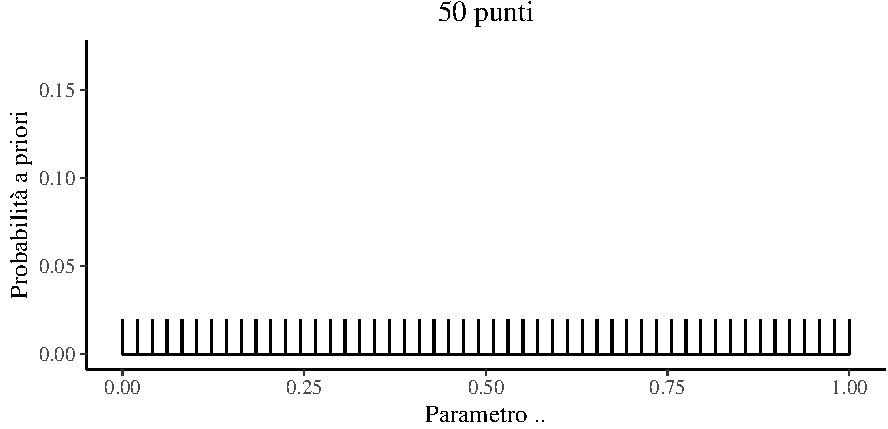
\includegraphics{910_grid_method_example_files/figure-latex/gridappr1-1} 

}

\caption{Rappresentazione grafica della distribuzione a priori per il parametro $   heta$, ovvero la probabilità di aspettative future distorte negativamente.}\label{fig:gridappr1}
\end{figure}

\hypertarget{funzione-di-verosimiglianza}{%
\section{Funzione di verosimiglianza}\label{funzione-di-verosimiglianza}}

Calcoliamo ora la funzione di verosimiglianza utilizzando i 50 valori \(\theta\) definiti in precedenza. A ciascuno dei valori della griglia applichiamo la formula binomiale, tendendo costanti i dati (ovvero 23 ``successi'' in 30 prove). Ad esempio, in corrispondenza del valore \(\theta = 0.816\), l'ordinata della funzione di verosimiglianza diventa

\begin{equation}
\binom{30}{23} \cdot 0.816^{23} \cdot (1 - 0.816)^{7} = 0.135.\notag
\end{equation}

\noindent
Per \(\theta = 0.837\), l'ordinata della funzione di verosimiglianza sarà

\begin{equation}
\binom{30}{23} \cdot 0.837^{23} \cdot (1 - 0.837)^{7} = 0.104.\notag
\end{equation}

\noindent
Dobbiamo svolgere questo calcolo per tutti gli elementi della griglia. Usando \(\R\), tale risultato si trova nel modo seguente:

\begin{Shaded}
\begin{Highlighting}[]
\NormalTok{likelihood }\OtherTok{\textless{}{-}} \FunctionTok{dbinom}\NormalTok{(}\AttributeTok{x =} \DecValTok{23}\NormalTok{, }\AttributeTok{size =} \DecValTok{30}\NormalTok{, }\AttributeTok{prob =}\NormalTok{ p\_grid)}
\NormalTok{likelihood}
\CommentTok{\#\textgreater{}  [1] 0.000000e+00 2.352564e{-}33 1.703051e{-}26 1.644169e{-}22}
\CommentTok{\#\textgreater{}  [5] 1.053708e{-}19 1.525217e{-}17 8.602222e{-}16 2.528440e{-}14}
\CommentTok{\#\textgreater{}  [9] 4.606907e{-}13 5.819027e{-}12 5.499269e{-}11 4.105534e{-}10}
\CommentTok{\#\textgreater{} [13] 2.520191e{-}09 1.311195e{-}08 5.919348e{-}08 2.362132e{-}07}
\CommentTok{\#\textgreater{} [17] 8.456875e{-}07 2.749336e{-}06 8.196948e{-}06 2.259614e{-}05}
\CommentTok{\#\textgreater{} [21] 5.798673e{-}05 1.393165e{-}04 3.148623e{-}04 6.720574e{-}04}
\CommentTok{\#\textgreater{} [25] 1.359225e{-}03 2.611870e{-}03 4.778973e{-}03 8.340230e{-}03}
\CommentTok{\#\textgreater{} [29] 1.390025e{-}02 2.214199e{-}02 3.372227e{-}02 4.909974e{-}02}
\CommentTok{\#\textgreater{} [33] 6.830377e{-}02 9.068035e{-}02 1.146850e{-}01 1.378206e{-}01}
\CommentTok{\#\textgreater{} [37] 1.568244e{-}01 1.681749e{-}01 1.688979e{-}01 1.575211e{-}01}
\CommentTok{\#\textgreater{} [41] 1.348746e{-}01 1.043545e{-}01 7.133007e{-}02 4.165680e{-}02}
\CommentTok{\#\textgreater{} [45] 1.972669e{-}02 6.936821e{-}03 1.535082e{-}03 1.473375e{-}04}
\CommentTok{\#\textgreater{} [49] 1.868105e{-}06 0.000000e+00}
\end{Highlighting}
\end{Shaded}

\noindent
La funzione \texttt{dbinom(x,\ size,\ prob)} richiede che vengano specificati tre parametri: il numero di ``successi'', il numero di prove e la probabilità di successo. Nella chiamata precedente, \texttt{x} (numero di successi) e \texttt{size} (numero di prove bernoulliane) sono degli scalari e \texttt{prob} è il vettore \texttt{p\_grid}. In tali circostanze, l'output di \texttt{dbinom()} è il vettore che abbiamo chiamato \texttt{likelihood}. Gli elementi di tale vettore sono stati calcolati applicando la formula della distribuzione binomiale a ciascuno dei 50 elementi della griglia, tenendo sempre costanti i dati {[}ovvero, \texttt{x} (il numero di successi) e \texttt{size} (numero di prove bernoulliane){]}; ciò che varia è il valore \texttt{prob}, che assume valori diversi (\texttt{p\_grid}) in ciascuna cella della griglia.

La chiamata a \texttt{dbinom()} produce dunque un vettore i cui valori corrispondono all'ordinata della funzione di verosimiglianza per per ciascun valore \(\theta\) specificato in \texttt{p\_grid}. La verosimiglianza discretizzata così ottenuta è riportata nella figura \ref{fig:gridappr2}.

\begin{Shaded}
\begin{Highlighting}[]
\NormalTok{p2 }\OtherTok{\textless{}{-}} \FunctionTok{data.frame}\NormalTok{(p\_grid, likelihood) }\SpecialCharTok{\%\textgreater{}\%}
  \FunctionTok{ggplot}\NormalTok{(}\FunctionTok{aes}\NormalTok{(}\AttributeTok{x=}\NormalTok{p\_grid, }\AttributeTok{xend=}\NormalTok{p\_grid, }\AttributeTok{y=}\DecValTok{0}\NormalTok{, }\AttributeTok{yend=}\NormalTok{likelihood)) }\SpecialCharTok{+}
  \FunctionTok{geom\_segment}\NormalTok{() }\SpecialCharTok{+}
  \FunctionTok{ylim}\NormalTok{(}\DecValTok{0}\NormalTok{, }\FloatTok{0.17}\NormalTok{) }\SpecialCharTok{+}
  \FunctionTok{labs}\NormalTok{(}
    \AttributeTok{x =} \StringTok{"Parametro \textbackslash{}U03B8"}\NormalTok{,}
    \AttributeTok{y =} \StringTok{"Verosimiglianza"}
\NormalTok{  )}
\NormalTok{p2}
\end{Highlighting}
\end{Shaded}

\begin{figure}

{\centering 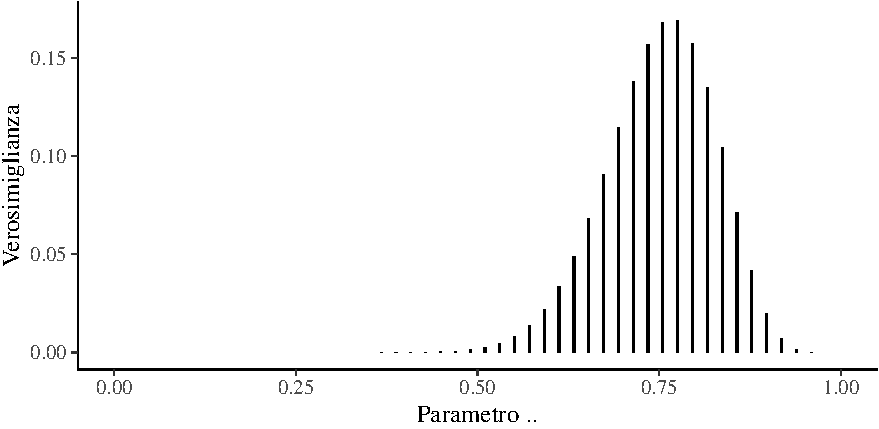
\includegraphics{910_grid_method_example_files/figure-latex/gridappr2-1} 

}

\caption{Rappresentazione della funzione di verosimiglianza per il parametro $\theta$, ovvero la probabilità di aspettative future distorte negativamente.}\label{fig:gridappr2}
\end{figure}

\hypertarget{distribuzione-a-posteriori-1}{%
\section{Distribuzione a posteriori}\label{distribuzione-a-posteriori-1}}

L'approssimazione discretizzata della distribuzione a posteriori \(p(\theta \mid y)\) si ottiene facendo il prodotto della verosimiglianza e della distribuzione a priori per poi scalare tale prodotto per una costante di normalizzazione. Il prodotto \(p(\theta)\mathcal{L}(y \mid \theta)\) produce la distribuzione a posteriori \emph{non standardizzata}.

Nel caso di una distribuzione a priori non informativa (ovvero una distribuzione uniforme), per ottenere la funzione a posteriori non standardizzata è sufficiente moltiplicare ciascun valore della funzione di verosimiglianza per 0.02. Per esempio, per il primo valore della funzione di verosimiglianza usato quale esempio poco sopra, abbiamo \(0.135 \cdot 0.02\); per il secondo valore dell'esempio abbiamo \(0.104 \cdot 0.02\); e così via. Possiamo svolgere tutti i calcoli usando \(\R\) nel modo seguente:\footnote{Ricordiamo il principio dell'aritmetica vettorializzata: i vettori \texttt{likelihood} e \texttt{prior1} sono entrambi costituiti da 50 elementi. Se facciamo il prodotto tra i due vettori otteniamo un vettore di 50 elementi, ciascuno dei quali uguale al prodotto dei corrispondenti elementi dei vettori \texttt{likelihood} e \texttt{prior1}.}

\begin{Shaded}
\begin{Highlighting}[]
\NormalTok{unstd\_posterior }\OtherTok{\textless{}{-}}\NormalTok{ likelihood }\SpecialCharTok{*}\NormalTok{ prior1}
\NormalTok{unstd\_posterior}
\CommentTok{\#\textgreater{}  [1] 0.000000e+00 4.705127e{-}35 3.406102e{-}28 3.288337e{-}24}
\CommentTok{\#\textgreater{}  [5] 2.107415e{-}21 3.050433e{-}19 1.720444e{-}17 5.056880e{-}16}
\CommentTok{\#\textgreater{}  [9] 9.213813e{-}15 1.163805e{-}13 1.099854e{-}12 8.211068e{-}12}
\CommentTok{\#\textgreater{} [13] 5.040382e{-}11 2.622390e{-}10 1.183870e{-}09 4.724263e{-}09}
\CommentTok{\#\textgreater{} [17] 1.691375e{-}08 5.498671e{-}08 1.639390e{-}07 4.519229e{-}07}
\CommentTok{\#\textgreater{} [21] 1.159735e{-}06 2.786331e{-}06 6.297247e{-}06 1.344115e{-}05}
\CommentTok{\#\textgreater{} [25] 2.718450e{-}05 5.223741e{-}05 9.557946e{-}05 1.668046e{-}04}
\CommentTok{\#\textgreater{} [29] 2.780049e{-}04 4.428398e{-}04 6.744454e{-}04 9.819948e{-}04}
\CommentTok{\#\textgreater{} [33] 1.366075e{-}03 1.813607e{-}03 2.293700e{-}03 2.756411e{-}03}
\CommentTok{\#\textgreater{} [37] 3.136488e{-}03 3.363497e{-}03 3.377958e{-}03 3.150422e{-}03}
\CommentTok{\#\textgreater{} [41] 2.697491e{-}03 2.087091e{-}03 1.426601e{-}03 8.331361e{-}04}
\CommentTok{\#\textgreater{} [45] 3.945339e{-}04 1.387364e{-}04 3.070164e{-}05 2.946751e{-}06}
\CommentTok{\#\textgreater{} [49] 3.736209e{-}08 0.000000e+00}
\end{Highlighting}
\end{Shaded}

Avendo calcolato i valori della funzione a posteriori non standardizzata è poi necessario dividere per una costante di normalizzazione. Nel caso discreto, trovare il denominatore del teorema di Bayes è facile: esso è uguale alla somma di tutti i valori della distribuzione a posteriori non normalizzata. Per i dati presenti, tale costante di normalizzazione è uguale a 0.032:

\begin{Shaded}
\begin{Highlighting}[]
\FunctionTok{sum}\NormalTok{(unstd\_posterior)}
\CommentTok{\#\textgreater{} [1] 0.0316129}
\end{Highlighting}
\end{Shaded}

La standardizzazione dei due valori usati come esempio è data da: \(0.135 \cdot 0.02 / 0.032\) e da \(0.104 \cdot 0.02 / 0.032\). Usiamo \(\R\) per svolgere questo calcolo su tutti i 50 valori di \texttt{unstd\_posterior} così che la somma dei 50 i valori di \texttt{posterior} sia uguale a 1.0:

\begin{Shaded}
\begin{Highlighting}[]
\NormalTok{posterior }\OtherTok{\textless{}{-}}\NormalTok{ unstd\_posterior }\SpecialCharTok{/} \FunctionTok{sum}\NormalTok{(unstd\_posterior)}
\NormalTok{posterior}
\CommentTok{\#\textgreater{}  [1] 0.000000e+00 1.488357e{-}33 1.077440e{-}26 1.040188e{-}22}
\CommentTok{\#\textgreater{}  [5] 6.666313e{-}20 9.649330e{-}18 5.442222e{-}16 1.599625e{-}14}
\CommentTok{\#\textgreater{}  [9] 2.914574e{-}13 3.681425e{-}12 3.479129e{-}11 2.597379e{-}10}
\CommentTok{\#\textgreater{} [13] 1.594406e{-}09 8.295316e{-}09 3.744893e{-}08 1.494410e{-}07}
\CommentTok{\#\textgreater{} [17] 5.350268e{-}07 1.739376e{-}06 5.185824e{-}06 1.429552e{-}05}
\CommentTok{\#\textgreater{} [21] 3.668548e{-}05 8.813904e{-}05 1.991986e{-}04 4.251792e{-}04}
\CommentTok{\#\textgreater{} [25] 8.599178e{-}04 1.652408e{-}03 3.023432e{-}03 5.276472e{-}03}
\CommentTok{\#\textgreater{} [29] 8.794033e{-}03 1.400820e{-}02 2.133450e{-}02 3.106310e{-}02}
\CommentTok{\#\textgreater{} [33] 4.321259e{-}02 5.736920e{-}02 7.255582e{-}02 8.719259e{-}02}
\CommentTok{\#\textgreater{} [37] 9.921545e{-}02 1.063963e{-}01 1.068538e{-}01 9.965619e{-}02}
\CommentTok{\#\textgreater{} [41] 8.532881e{-}02 6.602021e{-}02 4.512719e{-}02 2.635430e{-}02}
\CommentTok{\#\textgreater{} [45] 1.248015e{-}02 4.388601e{-}03 9.711744e{-}04 9.321354e{-}05}
\CommentTok{\#\textgreater{} [49] 1.181862e{-}06 0.000000e+00}
\end{Highlighting}
\end{Shaded}

\noindent 
Verifichiamo:

\begin{Shaded}
\begin{Highlighting}[]
\FunctionTok{sum}\NormalTok{(posterior)}
\CommentTok{\#\textgreater{} [1] 1}
\end{Highlighting}
\end{Shaded}

La distribuzione a posteriori così trovata non è altro che la versione normalizzata della funzione di verosimiglianza: questo avviene perché la distribuzione a priori uniforme non ha aggiunto altre informazioni oltre a quelle che erano già fornite dalla funzione di verosimiglianza. L'approssimazione discretizzata di \(p(\theta \mid y)\) che abbiamo appena trovato è riportata nella figura \ref{fig:gridappr3}.

\begin{Shaded}
\begin{Highlighting}[]
\NormalTok{p3 }\OtherTok{\textless{}{-}} \FunctionTok{data.frame}\NormalTok{(p\_grid, posterior) }\SpecialCharTok{\%\textgreater{}\%}
  \FunctionTok{ggplot}\NormalTok{(}\FunctionTok{aes}\NormalTok{(}\AttributeTok{x=}\NormalTok{p\_grid, }\AttributeTok{xend=}\NormalTok{p\_grid, }\AttributeTok{y=}\DecValTok{0}\NormalTok{, }\AttributeTok{yend=}\NormalTok{posterior)) }\SpecialCharTok{+}
  \FunctionTok{geom\_segment}\NormalTok{() }\SpecialCharTok{+}
  \FunctionTok{ylim}\NormalTok{(}\DecValTok{0}\NormalTok{, }\FloatTok{0.17}\NormalTok{) }\SpecialCharTok{+}
  \FunctionTok{labs}\NormalTok{(}
    \AttributeTok{x =} \StringTok{"Parametro \textbackslash{}U03B8"}\NormalTok{,}
    \AttributeTok{y =} \StringTok{"Probabilità a posteriori"}
\NormalTok{  )}
\NormalTok{p3}
\end{Highlighting}
\end{Shaded}

\begin{figure}

{\centering 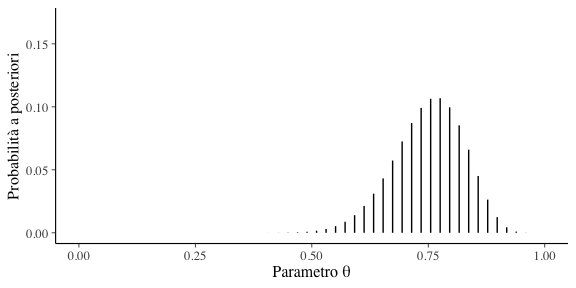
\includegraphics{910_grid_method_example_files/figure-latex/gridappr3-1} 

}

\caption{Rappresentazione della distribuzione a posteriori per il parametro $\theta$, ovvero la probabilità di aspettative future distorte negativamente.}\label{fig:gridappr3}
\end{figure}

I grafici delle figure \ref{fig:gridappr1}, \ref{fig:gridappr2} e \ref{fig:gridappr3} sono state calcolati utilizzando una griglia di 50 valori equi-spaziati per il parametro \(\theta\). I segmenti verticali rappresentano l'intensità della funzione in corrispondenza di ciascuna modalità parametro \(\theta\). Nella figura \ref{fig:gridappr1} e nella figura \ref{fig:gridappr3} la somma delle lunghezze dei segmenti verticali è uguale a 1.0; ciò non si verifica, invece, nel caso della figura \ref{fig:gridappr3} (la funzione di verosimiglianza non è mai una funzione di probabilità, né nel caso discreto né in quello continuo).

\hypertarget{es-depression-beta-2-10}{%
\section{La stima della distribuzione a posteriori (versione 2)}\label{es-depression-beta-2-10}}

Continuiamo l'analisi di questi dati esaminiamo l'impatto di una distribuzione a priori informativa sulla distribuzione a posteriori. Una distribuzione a priori informativa riflette un alto grado di certezza a priori sui valori dei parametri del modello. Un ricercatore utilizza una distribuzione a priori informativa per introdurre nel processo di stima informazioni pre-esistenti alla raccolta dei dati, introducendo così delle restrizioni sulla possibile gamma di valori del parametro.

Nel caso presente, supponiamo che la letteratura psicologica fornisca delle informazioni su \(\theta\) (la probabilità che le aspettative future di un individuo clinicamente depresso siano distorte negativamente). Per fare un esempio, supponiamo (irrealisticamente) che tali conoscenze pregresse possano essere rappresentate da una Beta di parametri \(\alpha = 2\) e \(\beta = 10\). Tali ipotetiche conoscenze pregresse ritengono molto plausibili valori \(\theta\) bassi e considerano implausibili valori \(\theta > 0.5\). Questo è equivalente a dire che ci aspettiamo che le aspettative relative all'umore futuro siano distorte negativamente solo per pochissimi individui clinicamente depressi --- ovvero, ci aspettiamo che la maggioranza degli individui clinicamente depressi sia inguaribilmente ottimista. Questa è, ovviamente, una credenza a priori del tutto irrealistica. La esamino qui, non perché abbia alcun senso nel contesto dei dati di \citet{zetschefuture2019}, ma soltanto per fare un esempio nel quale risulta chiaro come la distribuzione a posteriori sia una sorta di ``compromesso'' tra la distribuzione a priori e la verosimiglianza.

Con calcoli del tutto simili a quelli descritti sopra si giunge alla distribuzione a posteriori rappresentata nella figura \ref{fig:gridappr4}. Useremo ora una griglia di 100 valori per il parametro \(\theta\):

\begin{Shaded}
\begin{Highlighting}[]
\NormalTok{n\_points }\OtherTok{\textless{}{-}} \DecValTok{100}
\NormalTok{p\_grid }\OtherTok{\textless{}{-}} \FunctionTok{seq}\NormalTok{(}\AttributeTok{from =} \DecValTok{0}\NormalTok{, }\AttributeTok{to =} \DecValTok{1}\NormalTok{, }\AttributeTok{length.out =}\NormalTok{ n\_points)}
\end{Highlighting}
\end{Shaded}

\noindent
Per la distribuzione a priori scegliamo una Beta(2, 10):

\begin{Shaded}
\begin{Highlighting}[]
\NormalTok{alpha }\OtherTok{\textless{}{-}} \DecValTok{2}
\NormalTok{beta }\OtherTok{\textless{}{-}} \DecValTok{10}
\NormalTok{prior2 }\OtherTok{\textless{}{-}} \FunctionTok{dbeta}\NormalTok{(p\_grid, alpha, beta) }\SpecialCharTok{/} \FunctionTok{sum}\NormalTok{(}\FunctionTok{dbeta}\NormalTok{(p\_grid, alpha, beta))}
\FunctionTok{sum}\NormalTok{(prior2)}
\CommentTok{\#\textgreater{} [1] 1}
\end{Highlighting}
\end{Shaded}

\noindent
Tale distribuzione a priori è rappresentata nella figura \ref{fig:gridappr4}:

\begin{Shaded}
\begin{Highlighting}[]
\NormalTok{plot\_df }\OtherTok{\textless{}{-}} \FunctionTok{data.frame}\NormalTok{(p\_grid, prior2)}
\NormalTok{p4 }\OtherTok{\textless{}{-}}\NormalTok{ plot\_df }\SpecialCharTok{\%\textgreater{}\%}
  \FunctionTok{ggplot}\NormalTok{(}\FunctionTok{aes}\NormalTok{(}\AttributeTok{x=}\NormalTok{p\_grid, }\AttributeTok{xend=}\NormalTok{p\_grid, }\AttributeTok{y=}\DecValTok{0}\NormalTok{, }\AttributeTok{yend=}\NormalTok{prior2)) }\SpecialCharTok{+}
  \FunctionTok{geom\_segment}\NormalTok{() }\SpecialCharTok{+}
  \FunctionTok{ylim}\NormalTok{(}\DecValTok{0}\NormalTok{, }\FloatTok{0.17}\NormalTok{) }\SpecialCharTok{+}
  \FunctionTok{labs}\NormalTok{(}
    \AttributeTok{x =} \StringTok{""}\NormalTok{,}
    \AttributeTok{y =} \StringTok{"Probabilità a priori"}
\NormalTok{  )}
\NormalTok{p4}
\end{Highlighting}
\end{Shaded}

\begin{figure}

{\centering 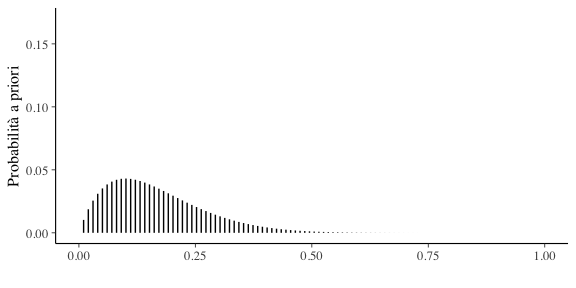
\includegraphics{910_grid_method_example_files/figure-latex/gridappr4-1} 

}

\caption{Rappresentazione di una funzione a priori informativa per il parametro $\theta$.}\label{fig:gridappr4}
\end{figure}

\noindent
Calcoliamo il valore di verosimiglianza per ciascun punto della griglia:

\begin{Shaded}
\begin{Highlighting}[]
\NormalTok{likelihood }\OtherTok{\textless{}{-}} \FunctionTok{dbinom}\NormalTok{(}\DecValTok{23}\NormalTok{, }\AttributeTok{size =} \DecValTok{30}\NormalTok{, }\AttributeTok{prob =}\NormalTok{ p\_grid)}
\end{Highlighting}
\end{Shaded}

\noindent
Per ciascun punto della griglia, il prodotto tra la verosimiglianza e distribuzione a priori è dato da:

\begin{Shaded}
\begin{Highlighting}[]
\NormalTok{unstd\_posterior2 }\OtherTok{\textless{}{-}}\NormalTok{ likelihood }\SpecialCharTok{*}\NormalTok{ prior2}
\end{Highlighting}
\end{Shaded}

\noindent
È necessario normalizzare la distribuzione a posteriori discretizzata:

\begin{Shaded}
\begin{Highlighting}[]
\NormalTok{posterior2 }\OtherTok{\textless{}{-}}\NormalTok{ unstd\_posterior2 }\SpecialCharTok{/} \FunctionTok{sum}\NormalTok{(unstd\_posterior2)}
\end{Highlighting}
\end{Shaded}

\noindent
Verifichiamo:

\begin{Shaded}
\begin{Highlighting}[]
\FunctionTok{sum}\NormalTok{(posterior2)}
\CommentTok{\#\textgreater{} [1] 1}
\end{Highlighting}
\end{Shaded}

\noindent
La nuova funzione a posteriori discretizzata è rappresentata nella figura \ref{fig:gridappr5}:

\begin{Shaded}
\begin{Highlighting}[]
\NormalTok{plot\_df }\OtherTok{\textless{}{-}} \FunctionTok{data.frame}\NormalTok{(p\_grid, posterior2)}
\NormalTok{p5 }\OtherTok{\textless{}{-}}\NormalTok{ plot\_df }\SpecialCharTok{\%\textgreater{}\%}
  \FunctionTok{ggplot}\NormalTok{(}\FunctionTok{aes}\NormalTok{(}\AttributeTok{x =}\NormalTok{ p\_grid, }\AttributeTok{xend =}\NormalTok{ p\_grid, }\AttributeTok{y =} \DecValTok{0}\NormalTok{, }\AttributeTok{yend =}\NormalTok{ posterior2)) }\SpecialCharTok{+}
  \FunctionTok{geom\_segment}\NormalTok{() }\SpecialCharTok{+}
  \FunctionTok{ylim}\NormalTok{(}\DecValTok{0}\NormalTok{, }\FloatTok{0.17}\NormalTok{) }\SpecialCharTok{+}
  \FunctionTok{labs}\NormalTok{(}
    \AttributeTok{x =} \StringTok{"Parametro \textbackslash{}U03B8"}\NormalTok{,}
    \AttributeTok{y =} \StringTok{"Probabilità a posteriori"}
\NormalTok{  )}
\NormalTok{p5}
\end{Highlighting}
\end{Shaded}

\begin{figure}

{\centering 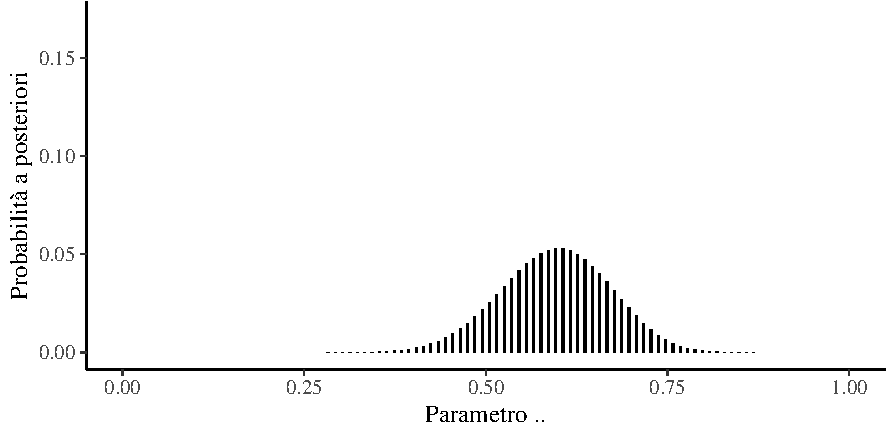
\includegraphics{910_grid_method_example_files/figure-latex/gridappr5-1} 

}

\caption{Rappresentazione della funzione a posteriori per il parametro $\theta$ calcolata utilizzando una distribuzione a priori informativa.}\label{fig:gridappr5}
\end{figure}

Facendo un confronto tra le figure \ref{fig:gridappr4} e \ref{fig:gridappr5} notiamo una notevole differenza tra la distribuzione a priori e la distribuzione a posteriori. In particolare, la distribuzione a posteriori risulta spostata verso destra su posizioni più vicine a quelle della verosimiglianza {[}figura \ref{fig:gridappr2}{]}. Si noti inoltre che, a causa dell'effetto della distribuzione a priori, le distribuzioni a posteriori delle figure \ref{fig:gridappr3} e \ref{fig:gridappr5} sono molto diverse tra loro.

Campioniamo ora 10,000 punti dall'approssimazione discretizzata della distribuzione a posteriori:

\begin{Shaded}
\begin{Highlighting}[]
\CommentTok{\# Set the seed}
\FunctionTok{set.seed}\NormalTok{(}\DecValTok{84735}\NormalTok{)}

\NormalTok{df }\OtherTok{\textless{}{-}} \FunctionTok{data.frame}\NormalTok{(}
\NormalTok{  p\_grid,}
\NormalTok{  posterior2}
\NormalTok{)}
\CommentTok{\# Step 4: sample from the discretized posterior}
\NormalTok{post\_samples }\OtherTok{\textless{}{-}}\NormalTok{ df }\SpecialCharTok{\%\textgreater{}\%}
  \FunctionTok{slice\_sample}\NormalTok{(}
  \AttributeTok{n =} \FloatTok{1e5}\NormalTok{,}
  \AttributeTok{weight\_by =}\NormalTok{ posterior2,}
  \AttributeTok{replace =} \ConstantTok{TRUE}
\NormalTok{)}
\end{Highlighting}
\end{Shaded}

\noindent
Una rappresentazione grafica del campione casuale estratto dalla distribuzione a posteriori \(p(\theta \mid y)\) è data da:

\begin{Shaded}
\begin{Highlighting}[]
\NormalTok{post\_samples }\SpecialCharTok{\%\textgreater{}\%}
  \FunctionTok{ggplot}\NormalTok{(}\FunctionTok{aes}\NormalTok{(}\AttributeTok{x =}\NormalTok{ p\_grid)) }\SpecialCharTok{+}
  \FunctionTok{geom\_histogram}\NormalTok{(}
    \FunctionTok{aes}\NormalTok{(}\AttributeTok{y =}\NormalTok{ ..density..), }
    \AttributeTok{color =} \StringTok{"white"}\NormalTok{, }
    \AttributeTok{binwidth =} \FloatTok{0.05}
\NormalTok{  ) }\SpecialCharTok{+}
  \FunctionTok{stat\_function}\NormalTok{(}\AttributeTok{fun =}\NormalTok{ dbeta, }\AttributeTok{args =} \FunctionTok{list}\NormalTok{(}\DecValTok{25}\NormalTok{, }\DecValTok{17}\NormalTok{)) }\SpecialCharTok{+}
  \FunctionTok{lims}\NormalTok{(}\AttributeTok{x =} \FunctionTok{c}\NormalTok{(}\DecValTok{0}\NormalTok{, }\DecValTok{1}\NormalTok{))}
\end{Highlighting}
\end{Shaded}

\begin{center}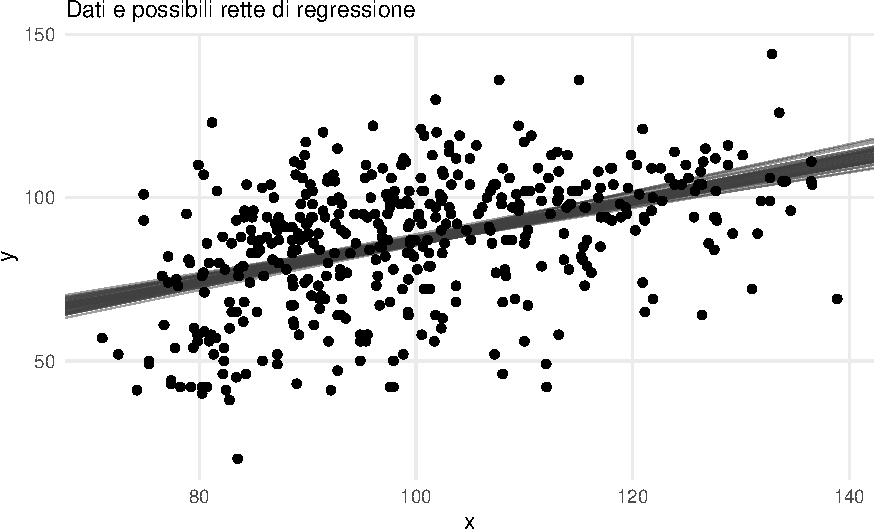
\includegraphics{910_grid_method_example_files/figure-latex/unnamed-chunk-16-1} \end{center}

\noindent
All'istogramma è stata sovrapposta la corretta distribuzione a posteriori, ovvero una Beta di parametri 25 (\(y + \alpha\) = 23 + 2) e 17 (\(n - y + \beta\) = 30 - 23 + 10).

La stima della moda a posteriori si ottiene con

\begin{Shaded}
\begin{Highlighting}[]
\NormalTok{df}\SpecialCharTok{$}\NormalTok{p\_grid[}\FunctionTok{which.max}\NormalTok{(df}\SpecialCharTok{$}\NormalTok{posterior2)]}
\CommentTok{\#\textgreater{} [1] 0.5959596}
\end{Highlighting}
\end{Shaded}

\noindent e corrisponde a

\[
\Mo = \frac{\alpha -1}{\alpha + \beta - 2} = \frac{25 - 1}{25 + 17 - 2} = 0.6.
\]

La stima della media a posteriori si ottiene con

\begin{Shaded}
\begin{Highlighting}[]
\FunctionTok{mean}\NormalTok{(post\_samples}\SpecialCharTok{$}\NormalTok{p\_grid)}
\CommentTok{\#\textgreater{} [1] 0.5953337}
\end{Highlighting}
\end{Shaded}

\noindent e corrisponde a

\[
\bar{\theta} = \frac{\alpha}{\alpha + \beta} = \frac{25}{25 + 17} \approx 0.5952.
\]

La stima della mediana a posteriori si ottiene con

\begin{Shaded}
\begin{Highlighting}[]
\FunctionTok{median}\NormalTok{(post\_samples}\SpecialCharTok{$}\NormalTok{p\_grid)}
\CommentTok{\#\textgreater{} [1] 0.5959596}
\end{Highlighting}
\end{Shaded}

\noindent e corrisponde a

\[
\Me = \frac{\alpha - \frac{1}{3}}{\alpha + \beta - \frac{2}{3}} \approx 0.5968.
\]

  \bibliography{refs.bib,book.bib,packages.bib}

\end{document}
